\documentclass{tufte-handout} % A4 paper and 11pt font size
\usepackage[activate={true,nocompatibility},final,tracking=true,kerning=true,spacing=true,factor=1100,stretch=10,shrink=10]{microtype}
\usepackage[T1]{fontenc} % Use 8-bit encoding that has 256 glyphs
\usepackage{mathpazo} % Use the Adobe Utopia font for the document - comment this line to return to the LaTeX default
\usepackage[english]{babel} % English language/hyphenation
\usepackage{amsmath,amsfonts,amsthm, amssymb} % Math packages
\usepackage{pgf,tikz}
\usetikzlibrary{positioning,matrix,arrows}
\usepackage{float}
\usepackage{tikz-cd}
\usepackage{caption}
\usepackage{stmaryrd}
\usepackage{multicol}
\usepackage{booktabs}
\usepackage{verbatim}
\usepackage{lipsum} % Used for inserting dummy 'Lorem ipsum' text into the template
\usepackage{sectsty} % Allows customizing section commands
\allsectionsfont{\normalfont \bfseries} % Make all sections centered, the default font and small caps
\usepackage{enumerate}
\usepackage{pythonhighlight}
\usepackage{fancyhdr} % Custom headers and footers
\pagestyle{fancyplain} % Makes all pages in the document conform to the custom headers and footers
\fancyhead{} % No page header - if you want one, create it in the same way as the footers below
\fancyfoot[L]{} % Empty left footer
\fancyfoot[C]{} % Empty center footer
\fancyfoot[R]{\thepage} % Page numbering for right footer
\renewcommand{\headrulewidth}{0pt} % Remove header underlines
\renewcommand{\footrulewidth}{0pt} % Remove footer underlines
\setlength{\headheight}{13.6pt} % Customize the height of the header
\allowdisplaybreaks

\usepackage{graphicx}
\usepackage{subcaption}


\usepackage{hyperref}
\hypersetup{  
	colorlinks=true,
	urlcolor=cyan,
}

\urlstyle{same}

% Turn on numbering for section and subsection headings
\setcounter{secnumdepth}{2}


\geometry{
	left=13mm, % left margin
	textwidth=130mm, % main text block
	marginparsep=8mm, % gutter between main text block and margin notes
	marginparwidth=55mm % width of margin notes
}
\fontsize{10}{20}\selectfont
%----------------------------------------------------------------------------------------
%	TITLE SECTION
%----------------------------------------------------------------------------------------

\title{	
	\normalfont\normalsize 
	{Melbourne University - Summer 2023} \\ [0pt] % Your university, school and/or department name(s)
	\huge Notes on state-space formulation of PTA problem% The assignment title
}\author{T. Kimpson} % Your name
\date{\vspace{-5pt}\normalsize\today} % Today's date or a custom date

\begin{document}
\justifying 
\maketitle


\pagenumbering{gobble} %turn off page numbering
\tableofcontents




\section{Preamble}


These notes collect some ideas around how to formulate the PTA data analysis as a state-space problem. \newline 

\noindent We will frequently reference previous works from A.Melatos, in particular Melatos 2018 (GR assignment UniMelb) and Melatos 2022 (private communication at UniMelb). \newline 

\noindent Geometric units ($c=\hbar = G = 1$) are used throughout, with the usual convention of Roman indices ($i,j$) for spatial indices. Note that $i$ is used for both labelling tensor indices and as the imaginary number - I trust the difference to be obvious from the context.\newline

\noindent These are rough notes - likely full of typos and undefined terms! Hopefully they are still understandable. \newline 


\section{Derivation of pulsar frequency modulation due to GW}
We want to know how the pulse frequency from a pulsar is influenced by a passing gravitational wave (GW). \newline 

\noindent We will consider the pulse frequency as a photon with covariant 4-momentum $p_{\mu}$  \footnote{See Melatos 2022 for nuances and discussion around this construction of "pulse train as photon"} \newline 

\noindent We take a gravitational plane wave that perturbs a background Minkowski spacetime as \footnote{c.f. Melatos 2018, Equation 1}
\begin{equation}
g_{\mu \nu} = \eta_{\mu \nu} + H_{\mu \nu} e^{i(\Omega(\bar{n} \cdot \bar{x} - t) + \Phi_0)	}
\end{equation}
where the GW has angular frequency $\Omega$, propagates in the $\bar{n}$-direction and has a phase offset of  $\Phi_0$. Note that we are free to choose our coordinate system such that $\Phi_0$ is the GW phase at $t=0$ \textit{at the Earth.}\footnote{This point is important, since the phase offset is then the same between multiple pulsars. See also Melatos 2022 PT12}. The amplitude tensor $H_{\mu \nu}$ has zero temporal components ($H_{0 \mu} = H_{\mu 0} = 0$) whilst the spatial part is
\begin{align}
	H_{ij} = h_+ e_{ij}^+(\bar{n}) + h_{\times} e_{ij}^{\times}(\bar{n})
\end{align}
\noindent Note that we use a convention where the amplitudes $h_{+,\times}$ label the \textit{constant} amplitudes of the gravitational plane wave. All time variation in the strain is a result of the exponential term $e^{i\Omega t}$. This is in contrast to the notation used by some authors \footnote{see e.g. arXiv:1003.0677} where the amplitudes include the time variability $h_{+,\times} = h_{+,\times}(t)$. The polarisation tensors $e_{ij}^{+,\times}$ are uniquely defined by the principal axes of the wave. \newline 


\subsection{Setting up the problem}
The frequency of a photon with 4-momentum $p_{\mu}$ recorded by an observer with 4-velocity $u^{\mu}$ is 
\begin{equation}
	\nu = p_{\alpha} u^{\alpha}
\end{equation}


\noindent We consider both our emitter and receiver to be stationary, such that  
\begin{equation}
u^{\alpha}|_{\rm emitter} = u^{\alpha}|_{\rm receiver} = (1,0,0,0)
\end{equation}



\noindent Consequently the frequency can be identified with the temporal component of the covariant 4-momentum,
\begin{equation}
\nu = p_t
\end{equation}


\noindent The expression for the evolution of the pulse frequency as measured by the observer on Earth is then,

\begin{equation}
	p_t(\tau)|_{\rm Earth} = p_t(t_0)|_{\rm source} + \int_{t = t_0}^{t=\tau} \dot{p}_t dt
	\end{equation}

\noindent where the overdot denotes a derivative w.r.t. $t$. Since the influence of the GW perturbation on $\dot{p}_t$ is small, we can relate the source emission and receiver times as $\tau = t_0 + d$ and consider the photon trajectory to be an unperturbed path. \footnote{See also e.g. Maggiore who takes the same approach...} \newline 


\noindent To complete our expression, we now just need to determine $\dot{p}_t$ and integrate it.


\subsection{Hamiltonian Mechanics}

The Hamiltonian in covariant notation can be written as 

\begin{equation}
H(x^{\mu}, p_{\mu}) = \frac{1}{2} g_{\mu \nu} p^{\mu} p^{\nu},
\end{equation}

\noindent which if we substitute in our expression for the perturbed metric is

\begin{equation}
H = \frac{1}{2} \eta_{\mu \nu} p^{\mu} p^{\nu} + \frac{1}{2} H_{ij}p^i p^j e^{i(\Omega(\bar{n} \cdot \bar{x} - t) + \Phi_0)	}
\end{equation}

\noindent Hamilton's equations are
\begin{equation}
\frac{dx^{\mu}}{d\lambda} = \frac{\partial H}{\partial p_{\mu}} , \, \, \frac{dp_{\mu}}{d \lambda} = -\frac{\partial H}{\partial x^{\mu}} 
\end{equation}

\noindent for affine parameter $\lambda$. The derivative of the temporal component of the covariant momenta is then,
\begin{equation}
\frac{d p_{t}}{d \lambda} = -\frac{i\Omega}{2} H_{ij}p^i p^j  e^{i(\Omega(\bar{n}\cdot \bar{x} - t))+\Phi_0}
\end{equation}
\footnote{This is equivalent to Melatos 2018, Eq 5 for the specific case of a GW propagating in the $z$-direction, with zero phase offset.}


\noindent Therefore the derivative w.r.t coordinate time $t$ is,
\begin{equation}
\dot{p}_t = \frac{d p_{t}}{d \lambda} \left(\frac{dt}{d\lambda}\right)^{-1} = \frac{d p_{t}}{d \lambda} \left(\frac{1}{p^t}\right)
\end{equation}
\noindent To make contact with Melatos 2022 it will prove useful to recognise that $p^{\mu} = \omega(1,-q^x,-q^y,-q^z)$ where $\bar{q}$ is the unit vector between the Earth and pulsar \footnote{similarly $\bar{x}(t) = -\bar{q}t$} and $\omega$ is the \textit{constant} photon angular frequency. Given the small effect of the GW perturbation, at first order we can identify $\omega$ as either the frequency at source or observer (see Melatos 2022, PT16). \newline 



\noindent Note that $\dot{p}_t$ is entirely a function of the GW perturbation. In the Minkowski case the spacetime is stationary and so $p_t$ should be conserved along the geodesic.  \newline 


\noindent Bringing this all together we can write $\dot{p}_t$ in a condensed form as,
\begin{equation}
\dot{p}_t = A e^{i \gamma t + \Phi_0}
\end{equation}
where 
\begin{equation}
\gamma = -\Omega (1 + \bar{n}\cdot \bar{q}) 
\end{equation}
\footnote{compare with Melatos 2022, PT11}
\noindent and
\begin{equation}
A = -\frac{i\Omega \omega}{2} H_{ij}q^i q^j 
\end{equation}
where the $\omega$ term in the numerator results from a $\omega^2$ terms that comes from the $p^i p^j$ term and a $\omega^{-1}$ term from $(p^t)^{-1}$.
\subsection{Performing the integral}

The frequency shift experienced by the observer relative to the source due to a GW is then
\begin{align}
p_t(\tau)|_{\rm Earth} - p_t(\tau - d)|_{\rm source} = A \int_{t = \tau - d}^{t=\tau} e^{i \gamma t + \Phi_0}dt  \\
=\frac{-iA}{\gamma} e^{i \gamma \tau}e^{\Phi_0}[1 - e^{-i \gamma d}] 
\label{eq:concise}
\end{align}

\subsection{Explicit expression and comparison with Melatos 22}

We can expand the concise expression of Eq. \ref{eq:concise} as,

\begin{equation} \label{eq:final}
p_t(\tau)|_{\rm Earth} - p_t(\tau - d)|_{\rm source} =\frac{ \omega}{2} \frac{H_{ij}q^i q^j  }{(1 + \hat{n} \cdot \hat{q})}e^{-i \Omega \tau(1+\bar{n} \cdot \bar{q}) + \Phi_0} [1 - e^{i \Omega(1+\bar{n} \cdot \bar{q}) d}]
\end{equation}
This expression is equivalent to Melatos 2022, PT13 where the dependence on time $t$ is made explicit. Using the Melatos notation where $h_{ij} = g_{ij} - \eta_{ij}$


\begin{equation}
	p_t(\tau)|_{\rm Earth} - p_t(\tau - d)|_{\rm source} =\frac{ \omega}{2} \frac{h_{ij} q^i q^j  }{(1 + \hat{n} \cdot \hat{q})} [1 - e^{i \Omega(1+\bar{n} \cdot \bar{q}) d}]
\end{equation}

\newpage
\section{State-space structure} \label{sec3}
\noindent The general structure of a Kalman state-space problem is
\begin{equation}
	\dot{x} = f(x) + w
\end{equation}
where $x$ are the state variables, $f()$ a non-linear function of the states, and $w$ a stochastic zero-mean process. The process noise matrix $Q = E(w w^T)$. The states are related to the measurement $z$ via a non-linear measurement function $h()$
\begin{equation}
	z = h(x) + v
\end{equation}
where $v$ is a stochastic zero-mean process and measurement noise matrix $R = E(v v^T)$. \newline 


\noindent This structure maps onto the preceding equations nicely. Our hidden state is just the intrinsic pulsar frequency, which evolves as,
\begin{eqnarray}
	\dot{f}_P = -\gamma f_P^n + \xi(t)
\end{eqnarray}
where $n$ is a braking index (typical values $\sim 1-5$, we take a canonical value $=3$) \footnote{See A. Vargas talk re anomalous braking indices. P.S. is there an arXiv preprint?} $\gamma$ a proportionality constant, and $\xi(t)$ represents a stochastic white noise process. Equation \ref{eq:final} can be used to relate the intrinsic pulsar frequency to that measured by an observer on Earth:

\begin{eqnarray}
	f_M = f_p(1 - X) + N_M
\end{eqnarray}
where $X$ is the RHS of Eq. \ref{eq:final} and $N_M$ a Gaussian measurement noise. An example of the evolution of the state and the measurement frequencies for our PTA pulsars can be seen in Fig. \ref{fig:mean and std of nets}







\subsection{A note on magnitudes}

It is worth pausing to consider some typical values of our state/measurement variables, as well as the respective noises. 


\begin{itemize}
	\item $f_p$ - PTAs typically deal with millisecond pulsars. We can take a standard value of $f_P = 100$ Hz.
	\item $\gamma, n$ - These two parameters describe the secular spin down. We can take $n=3$ as a standard value (spindown due to dipole emission). It follows that $\gamma$ is of the order $10^{-23}$ for typical PTA pulsars (e.g. PSR J$0023+0923$ has $f\sim 330$ Hz and $\dot{f} \sim 10^{-15} s^{-2}$)
	\item $\sigma_p$ - this is the parameter which quantifies the strength of  $\xi(t)$ i.e. the pulsar red noise (sometimes known as timing noise). For MSPs the red noise is typically small - we can set it to be some fraction of $\dot{f}$ e.g. if 10$\%$ then $\sigma_p \sim 10^{-16}$.
	\item $X$ - The magnitude of $X$ is set by the GW amplitude, which is expected to be $\lesssim 10^{-15}$ 
	\item $\sigma_m$ - this is the parameter which quantifies the strength of the Gaussian measurement noise i.e. the radiometer white noise. Typical measurement uncertainty in the pulsar TOAs is $\sim 10 - 100$ ns for our best MSPs. If we take an observation cadence of $\sim 1$ month then we can relate the uncertainty in the TOA to the uncertainty in the frequency as $\sigma_m / f \sim 10 \text{ns} / 1 \text{ month}  \sim 4 \times 10^{-15}$. \footnote{L.Dunn gave some good advice on how this works, but I am still a bit unsure whether this quite makes sense?}
\end{itemize}


\begin{figure}
	\centering
	\begin{subfigure}[b]{0.475\textwidth}
		\centering
		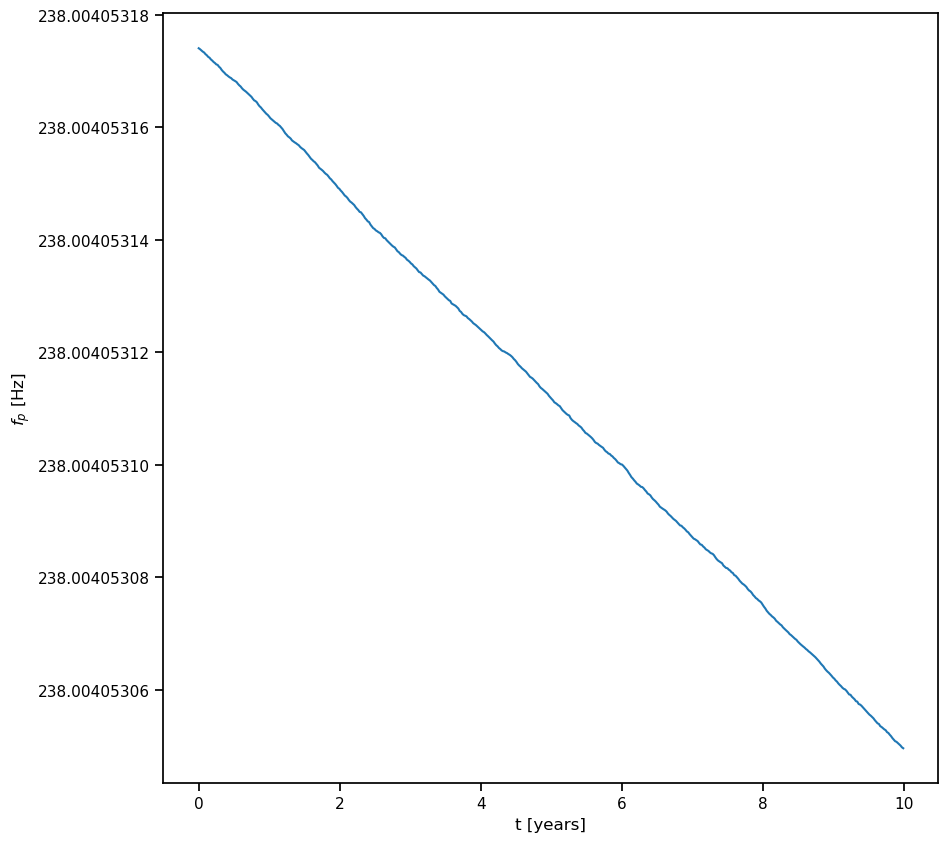
\includegraphics[width=\textwidth]{images/fp1}
		\caption{State frequency, single pulsar}%
		   
		\label{fig:mean and std of net14}
	\end{subfigure}
	\hfill
	\begin{subfigure}[b]{0.475\textwidth}  
		\centering 
		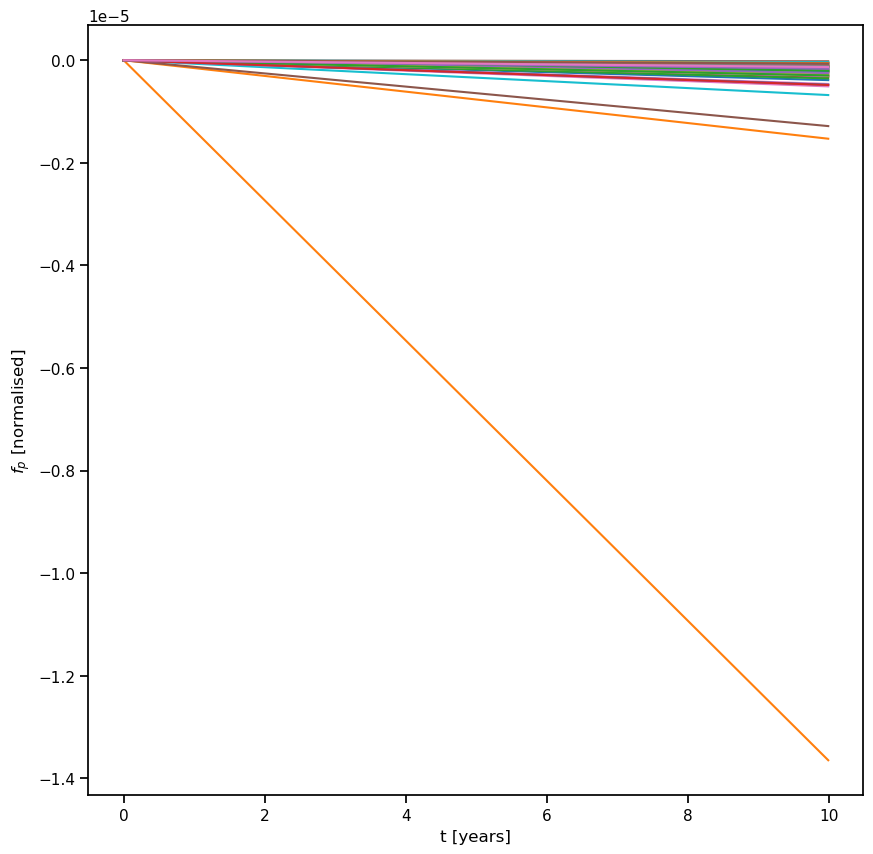
\includegraphics[width=\textwidth]{images/fp_all}
		\caption{State frequency, multiple pulsars}
		\label{fig:mean and std of net24}
	\end{subfigure}
	\vskip\baselineskip
	\begin{subfigure}[b]{0.475\textwidth}   
		\centering 
		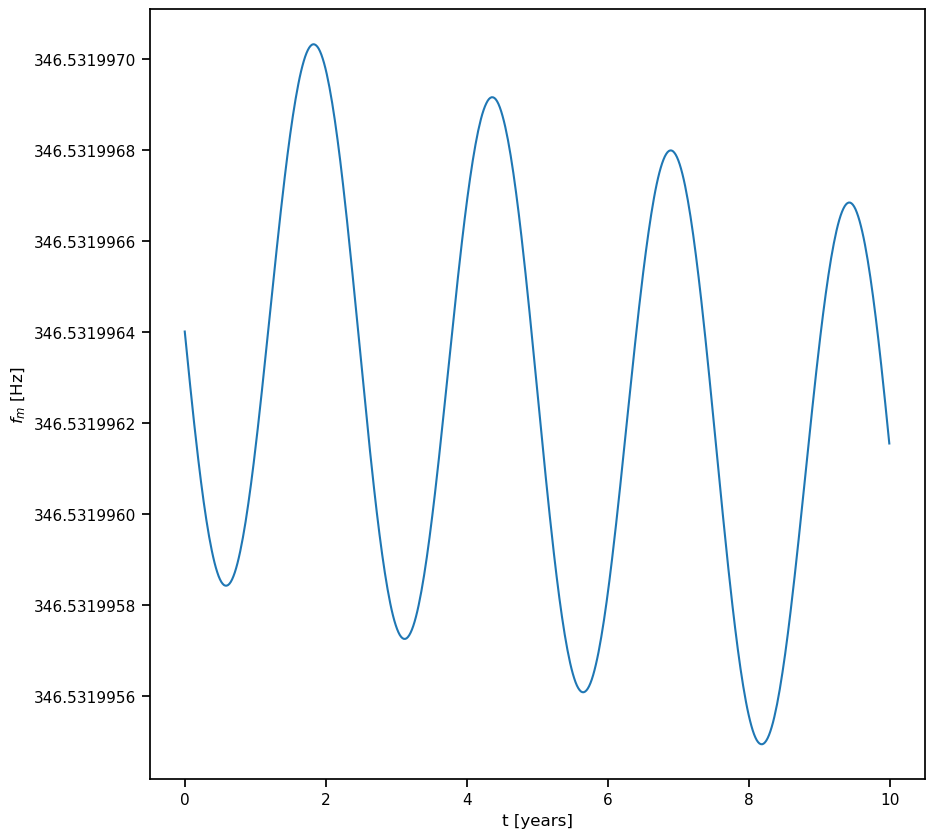
\includegraphics[width=\textwidth]{images/fm1}
		\caption{Measured frequency, single pulsar}  
		\label{fig:mean and std of net34}
	\end{subfigure}
	\hfill
	\begin{subfigure}[b]{0.475\textwidth}   
		\centering 
		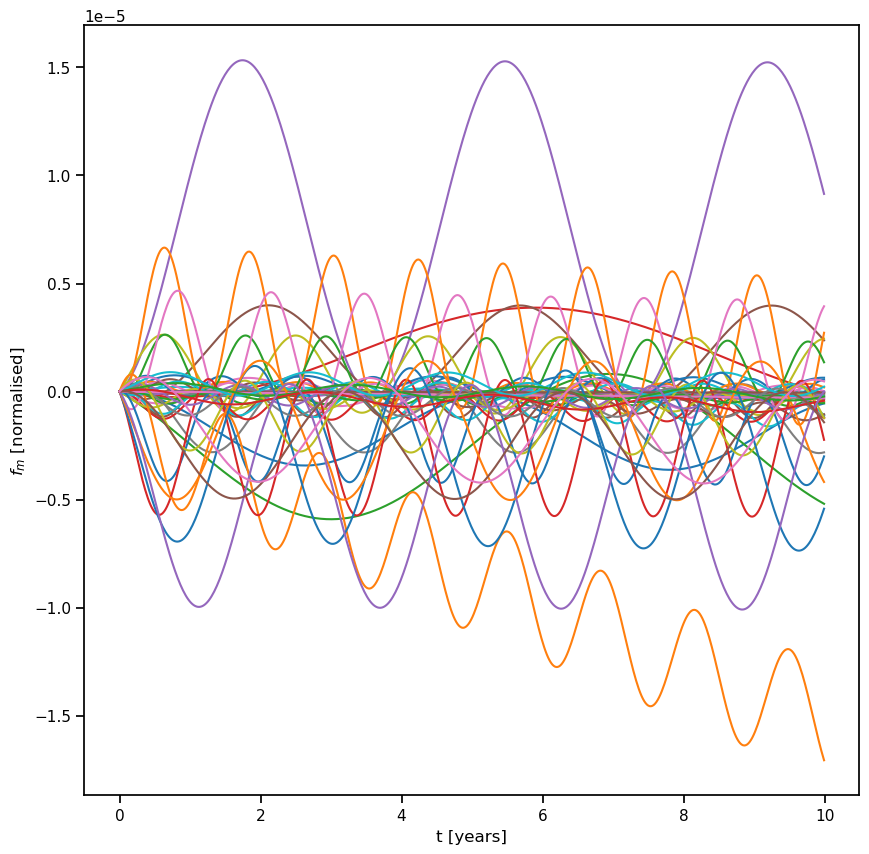
\includegraphics[width=\textwidth]{images/fm_all}
		\caption{Measured frequency, multiple pulsars}   
		\label{fig:mean and std of net44}
	\end{subfigure}
	\caption{Evolution of the state (top row) and measurement (bottom row) frequencies for pulsars influenced by an arbitrary GW source.}
	\label{fig:mean and std of nets}
\end{figure}


\newpage
\section{Constructing a PTA}\label{sec:PTA}


In order to proceed and explore how well this state-space formulation works, we will need to specify a selection of pulsars to make up our PTA. We will take the 47 pulsars that make up the NANOGrav PTA \footnote{Data obtained from the ANTF catalogue at \url{https://www.atnf.csiro.au/research/pulsar/psrcat/}} \newline  



\noindent ANTF provides values for both $f$ and $\dot{f}$. For every pulsar we will assume that $n=3$ and calculate $\gamma$ accordingly. For example, PSR J1713+0747 has a spin frequency of 218 Hz and a derivative $-4 \times 10^{-16}$ s $^{-2}$. Taking $n=3$ gives $\gamma \sim 3.9 \times 10^{-23}$. \newline 


\noindent Approximate pulsar distances are also provided. For now we will take these as known rather than additional parameters to be inferred. The median pulsar distance for NANOGrav pulsars is $\sim 1.3$ kpc. The distribution of NANOGrav pulsars on the sky is shown in Fig \ref{fig:pulsar_distrib}



\begin{figure}
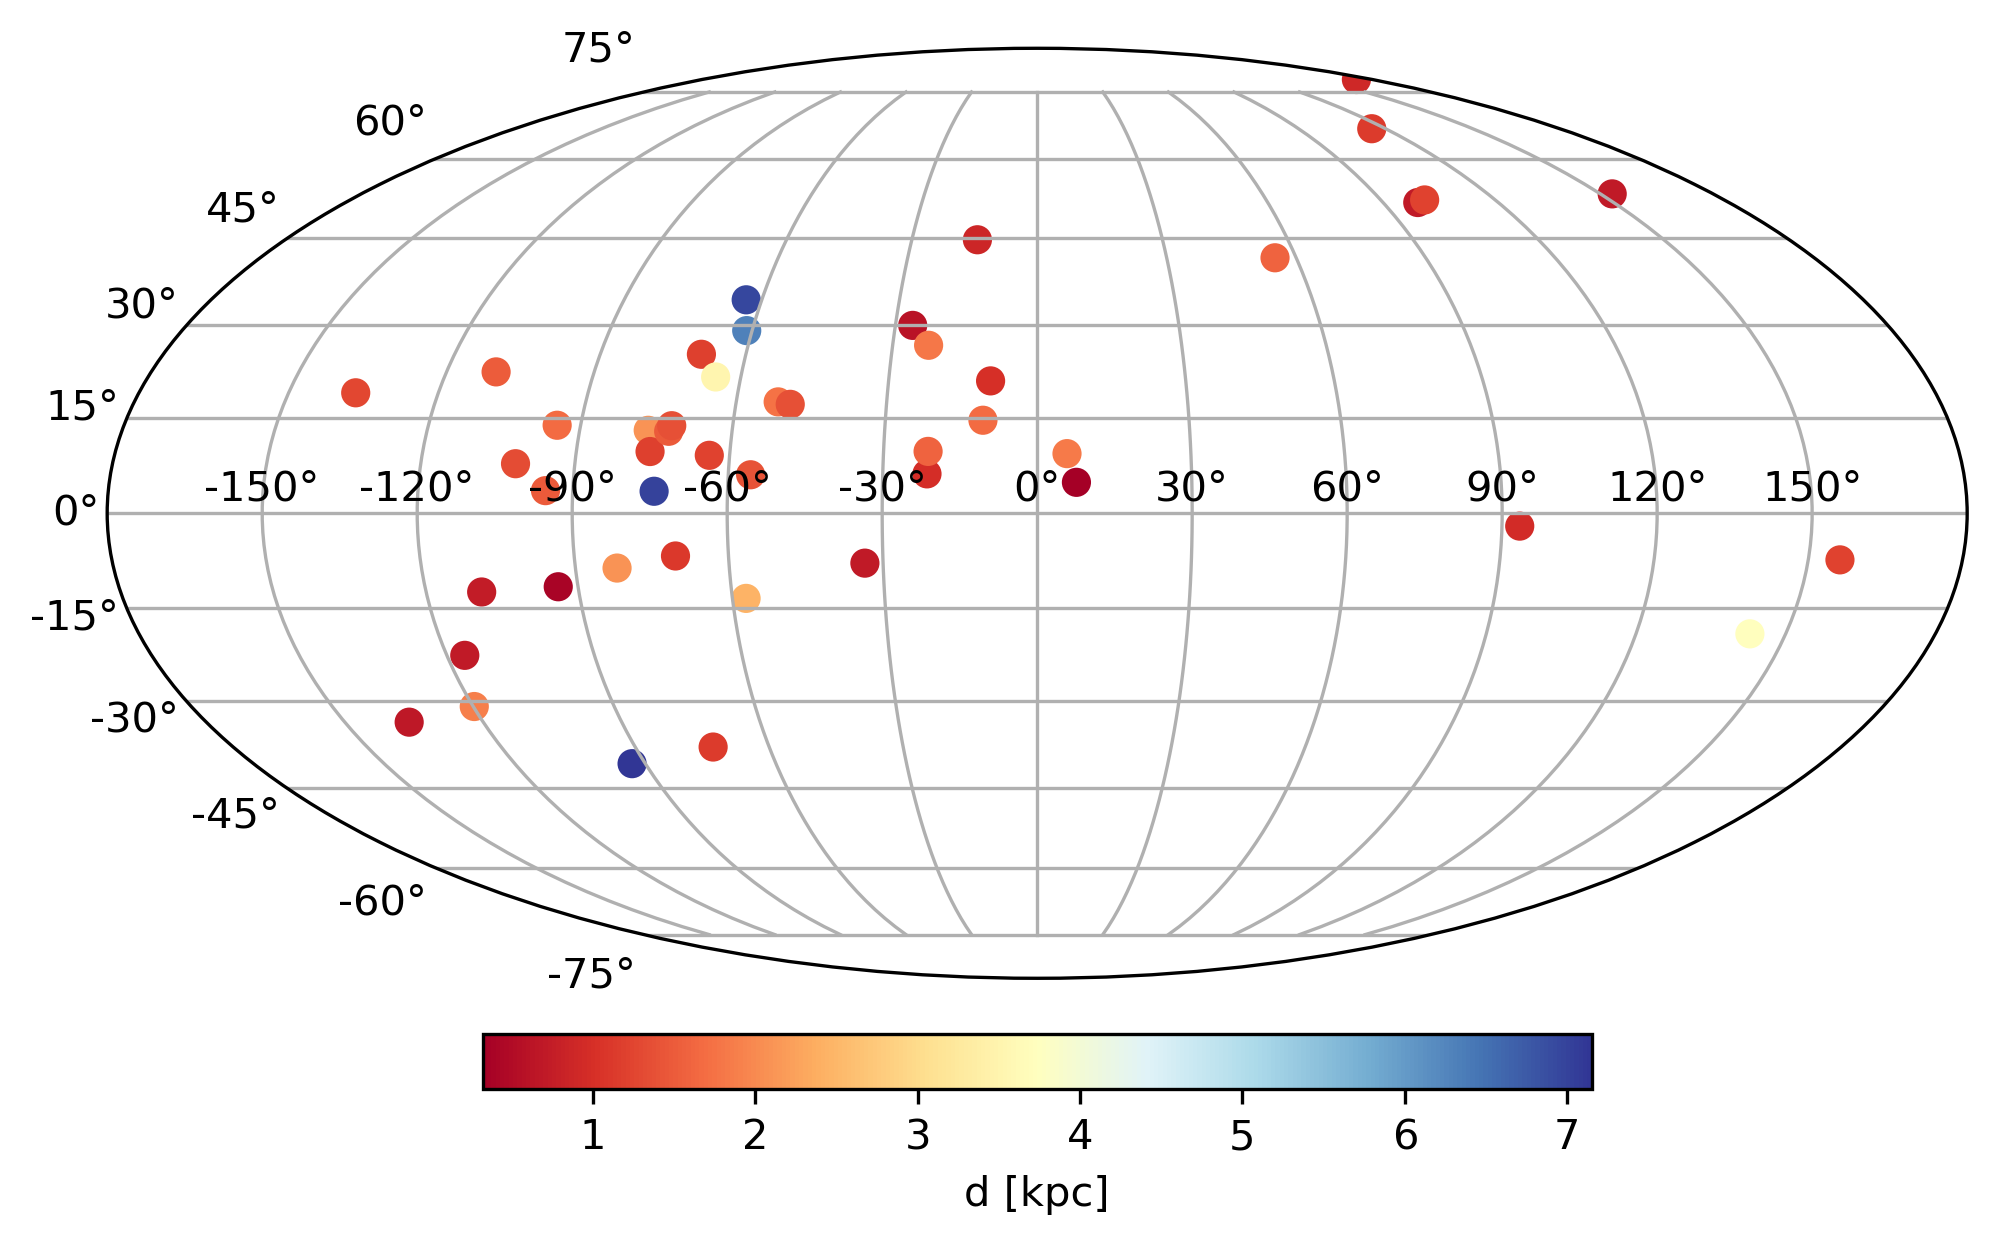
\includegraphics[width=0.8\textwidth]{images/pulsars}
\caption{Spatial distribution and distances of NANOGrav pulsars}
\label{fig:pulsar_distrib}
\end{figure}


\newpage 
\section{Model selection using a UKF}
\noindent We can construct some noisy synthetic data using the equations and values of Section \ref{sec3} and then apply an unscented Kalman filter \footnote{See \href{https://groups.seas.harvard.edu/courses/cs281/papers/unscented.pdf}{Wan \& van der Merwe} for a very readable description of how the UKF works } to the measured frequency to try to recover the intrinsic state frequency. An example of this is shown below in Fig \ref{fig:model example} below for some large GW strain. We can see that for this example the filter can recover the state evolution well. 

\begin{figure}
	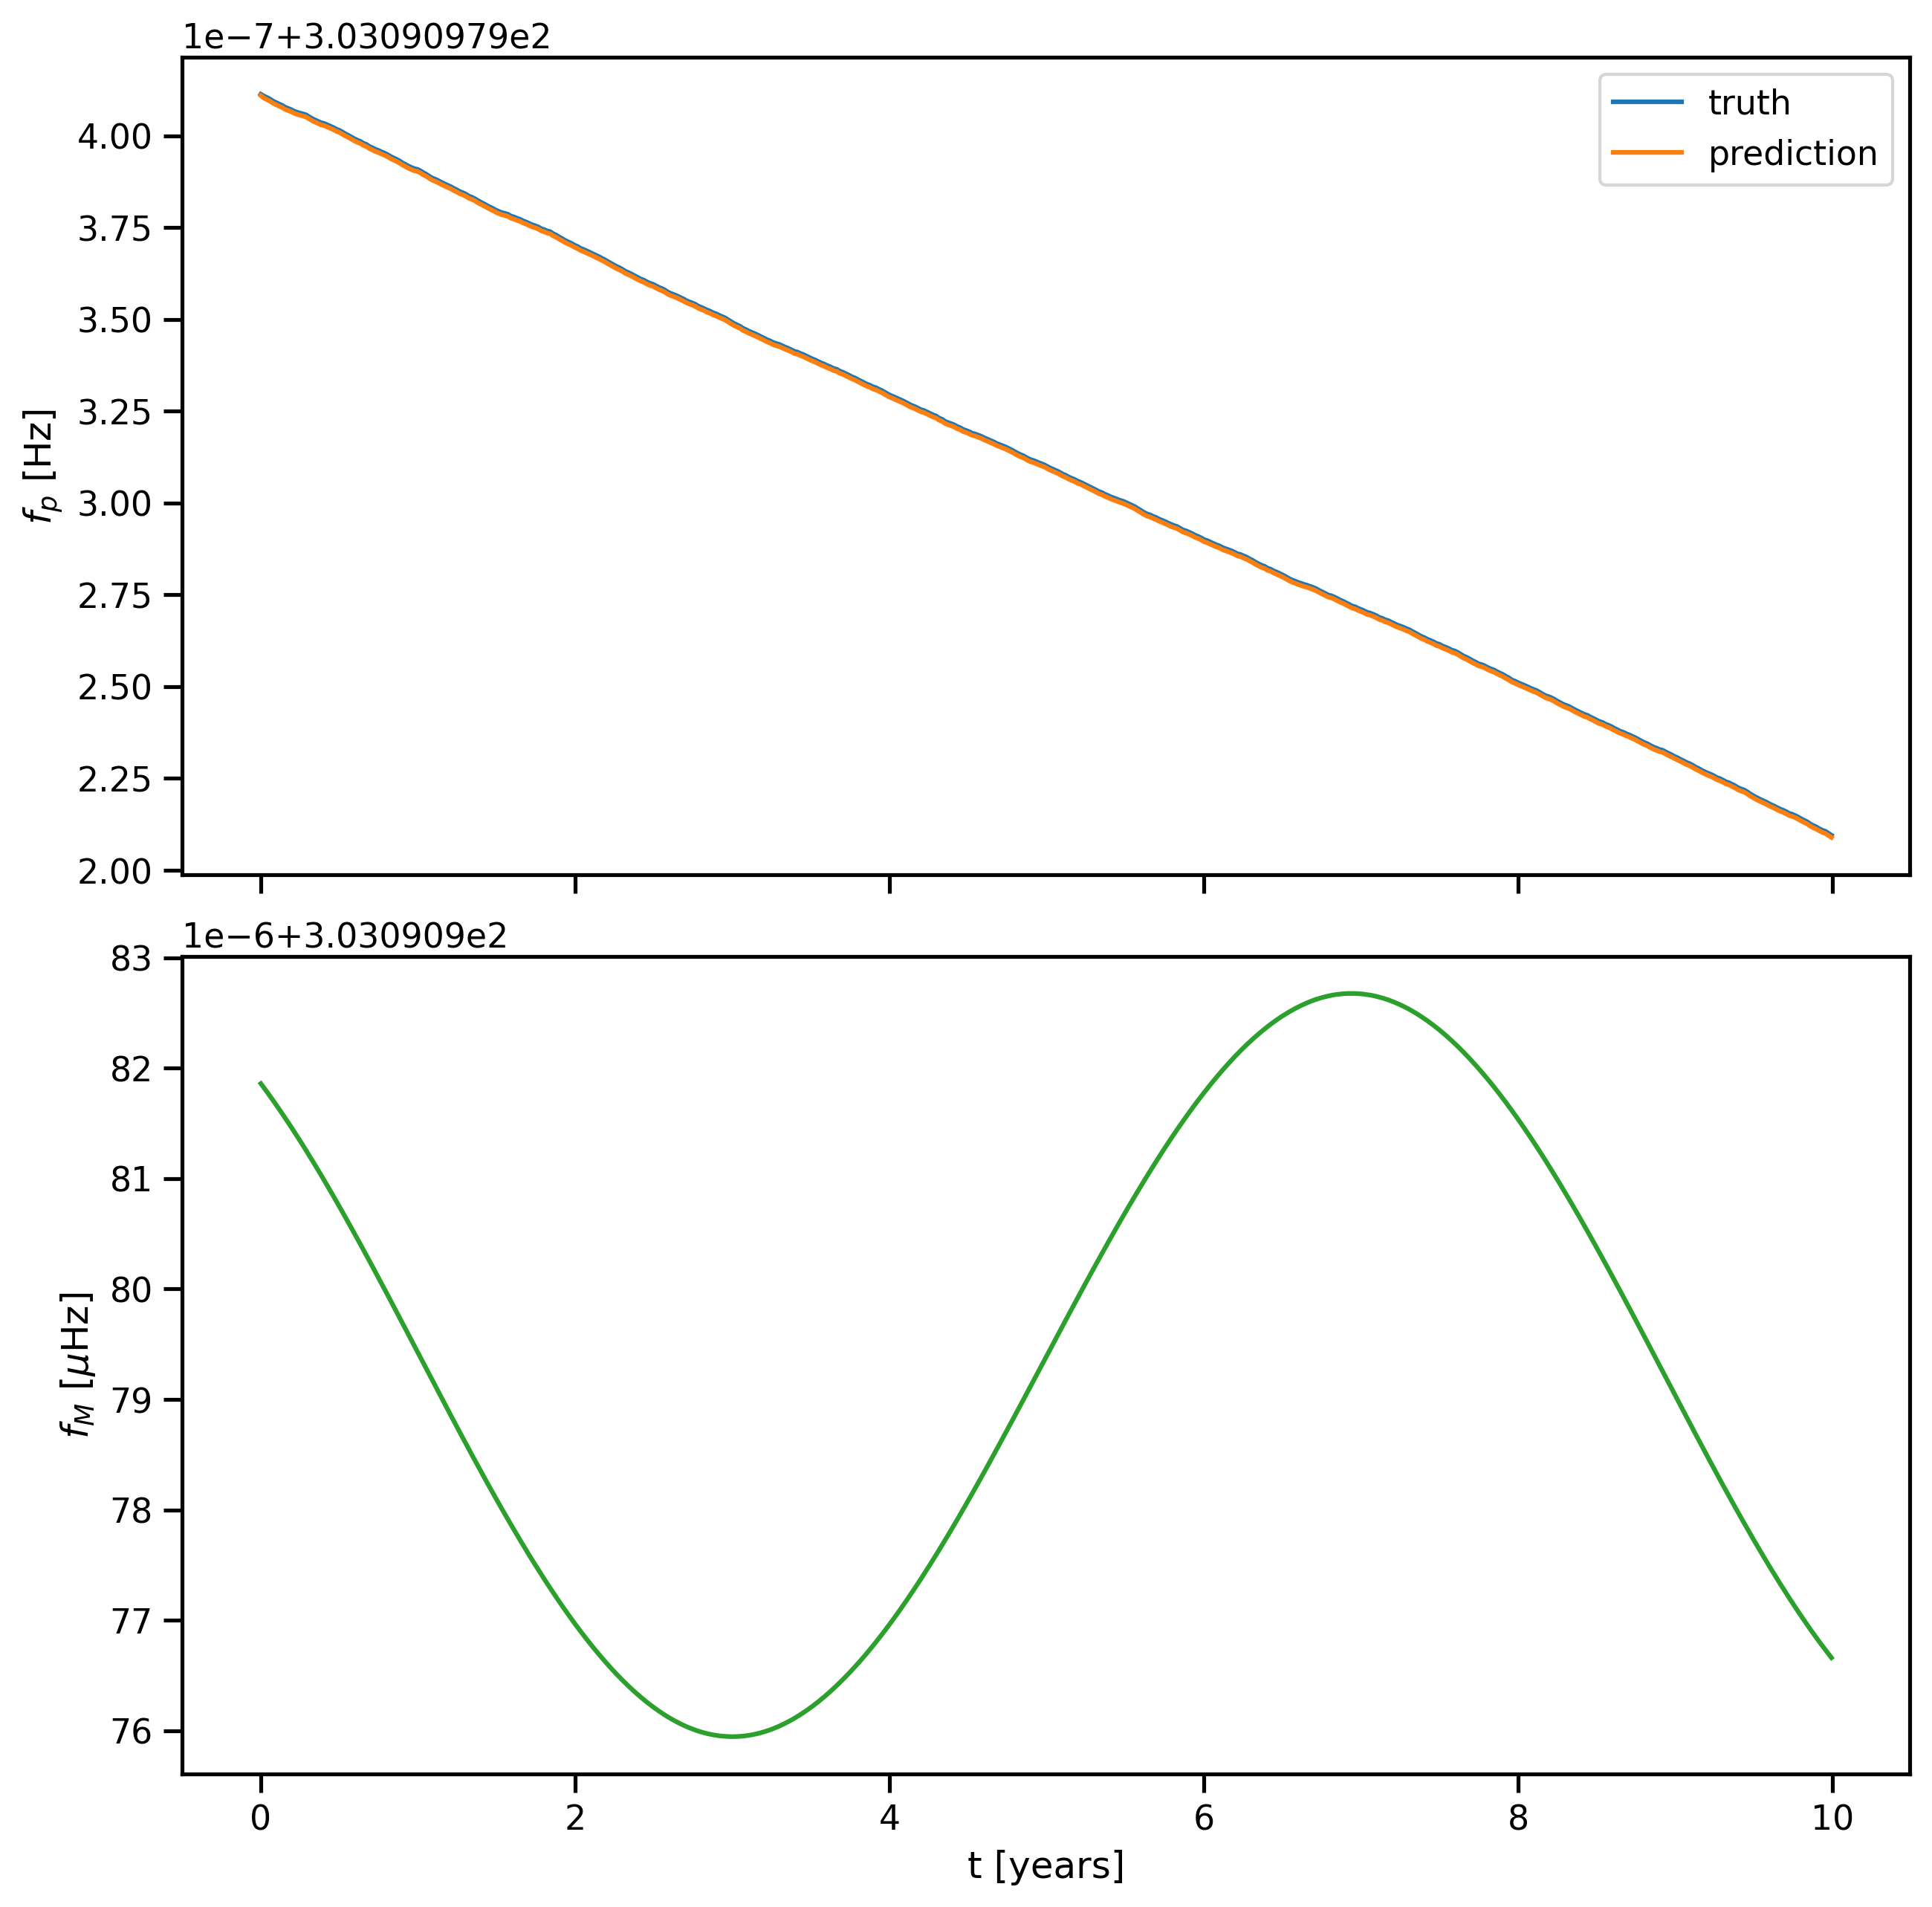
\includegraphics[width=0.8\textwidth]{images/model}
	\caption{Recovery of the pulsar state frequency from the measurement frequency by a UKF.}
	\label{fig:model example}
\end{figure}
\noindent We can use this UKF to try to solve the problem of GW detection i.e. \textit{"Is there evidence of a GW in my data?}. We can frame this as a model selection procedure where we have two models/hypotheses:

\begin{itemize}
	\item \textbf{Null Model} $M_0$. There is no GW in the data. In this case the measurement model of the UKF simply returns the frequency states (i.e. $X= 0$)
	\item \textbf{Alternative model} $M_1$. There is a GW in the data. The measurement model uses the full expression for $X$
\end{itemize}
\begin{figure}
	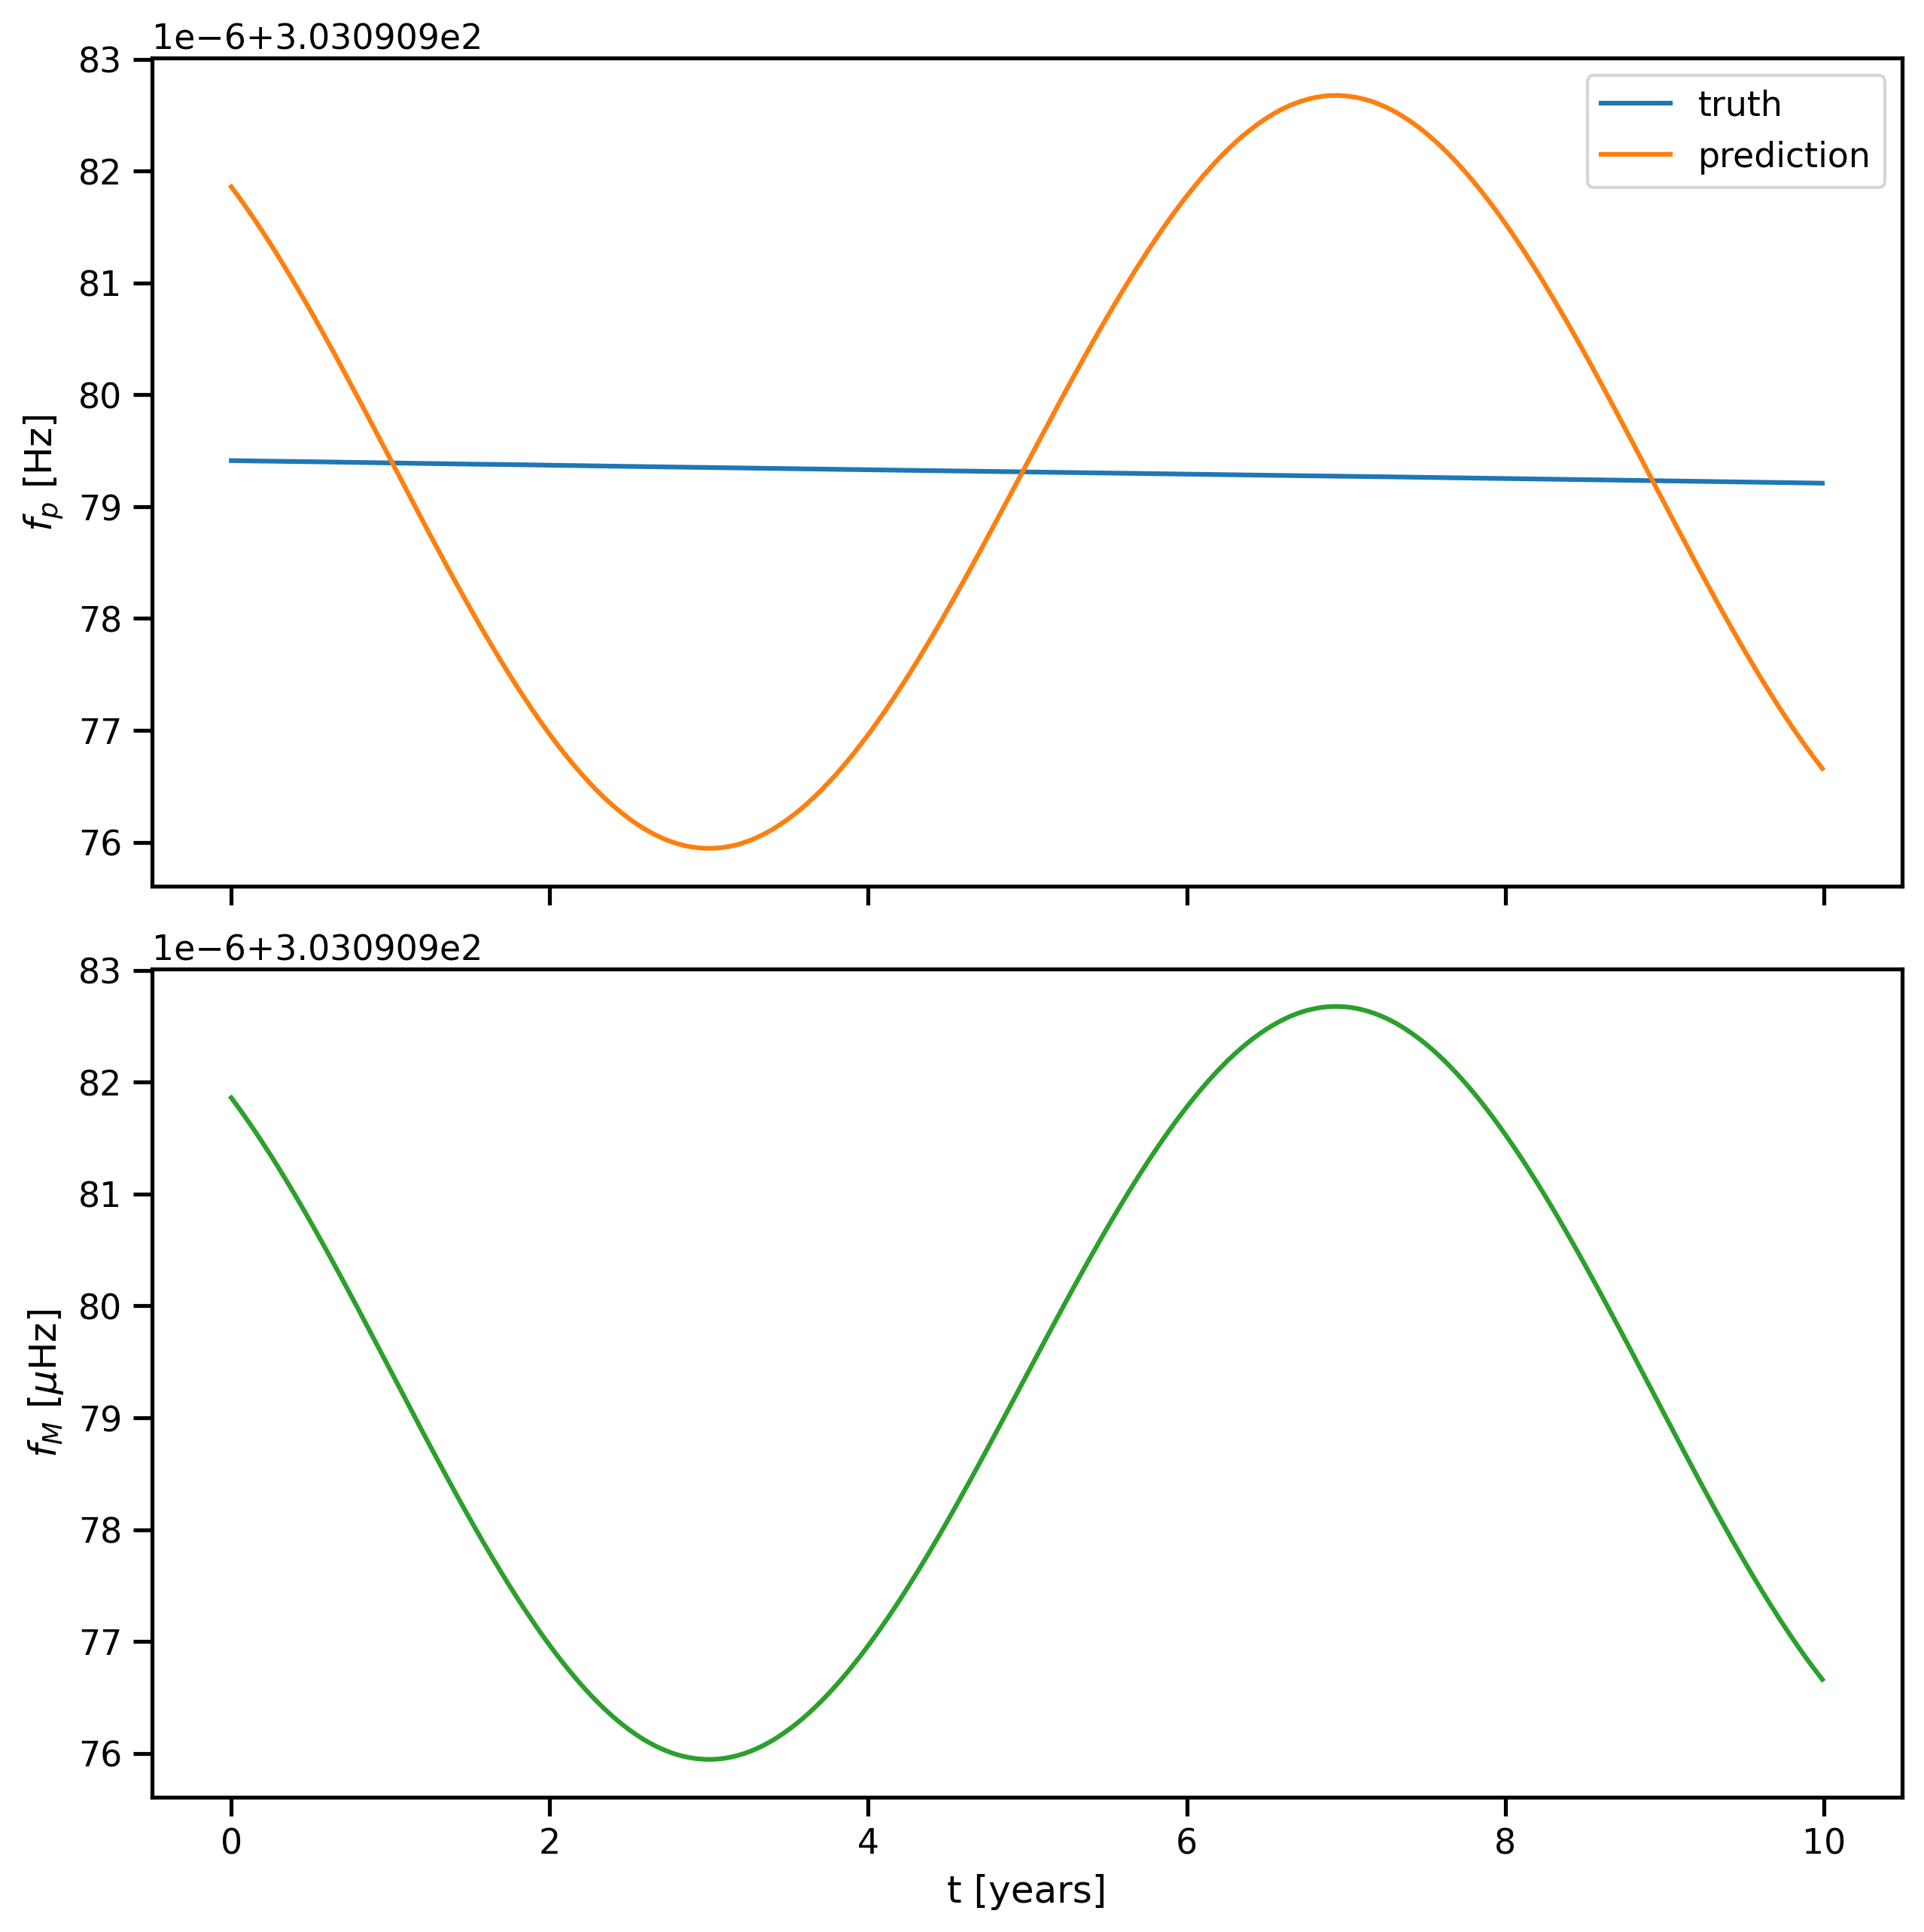
\includegraphics[width=0.8\textwidth]{images/null}
	\caption{As Fig 3, but now for a the null model. The state is not well recovered.}
	\label{fig:null example}
\end{figure}
\noindent An example applying the null model to the same data as in Fig \ref{fig:model example} is shown in Fig \ref{fig:null example}. Evidently the null model does not capture the true underlying state well. \newline 

\noindent In order to accept the alternative hypothesis $M_1$ over $M_0$ there are two approaches we could take:
\begin{itemize}
	\item The first is a fully Bayesian search over all the parameters for each model, calculating the evidence for each model and then determining the Bayes ratio. This is perhaps the most consistent way, but it is obviously expensive and at this stage we are keen to explore how detectability varies with e.g. GW strain.
	\item The second method is to recognize that $M_0$ and $M_1$ are hierarchically nested models and we can perform a likelihood ratio test. That is, given the maximum likelihood estimators $\hat{\theta}$ of the true parameters $\theta$, the likelihood of each model can be calculated and compared. These likelihoods are just  point estimates of the Bayes factor numerator/denominators.
\end{itemize}
Given the cheap cost we proceed with the second method.


\subsection{Likelihood ratio test}
For the likelihood ratio test we do not perform any kind of maximum likelihood search over the parameters for each of the models. Instead we just artificially set the maximum likelihood estimators to be equal to the true parameters of the system \footnote{i.e. $\hat{\theta} = \theta$}. We assume that any maximum likelihood algorithm would converge to these parameters \footnote{This is obviously an oversimplification but will serve our purposes for now}. \newline  


\noindent Interpreting the likelihood ratio $\Lambda$ also needs some consideration, since we have to account for the increased model complexity of $M_1$ \footnote{Bayes factors penalise complexity by construction since one must integrate over a larger parameter space}. This can be accomplished via Wilks' Theorem which states that for a large nuber of samples \footnote{What counts as large? See \url{https://www.osti.gov/servlets/purl/1529145}} the distribution of the test statistic approaches the chi-squared distribution under the null hypothesis i.e. 
\begin{equation}
2 \log \Lambda \rightarrow \chi^2
\end{equation}
One can then compute $p$-values where the number of degrees of freedom is equal to the difference in the number of parameters of the two models; $M_1$ has 7 extra parameters over $M_0$

\begin{itemize}
	\item Parameters $M_0$: $\gamma$, $n$
	\item Parameters $M_1$: $\gamma$, $n$, $\omega$, $\theta$, $\phi$, $\psi$, $\iota$, $\Phi_0$,$h$
\end{itemize}
With 7 degrees of freedom and a target tolerance of 5(1) \% the test statistic is $\sim 14 (18.5)$. For the toy system exhibited in Figs. \ref{fig:model  example}, \ref{fig:null example}, the test statistic is $\gg 20$ - this makes intuitive sense since it is immediately obvious to the eye that the data is sinusoidal. But what about other systems? 


\subsection{Detectability vs strain}

Lets take a system and explore how the detectability, as quantified by the test statistic varies with GW strain. For our PTA we use the NANOGrav pulsars described in Section \ref{sec:PTA}, with an observation length of 10 years and a weekly cadence. The GW source parameters are listed in Table \ref{tab:toy_example_parameters}. The results for this system are presented in Figure \ref{fig:SNR}, for a single noise realisation. We consider both the test statistic, $2 \log \Lambda$, and another parameter $\delta$ which is the median absolute error in the state estimates \footnote{In real-life we of course cannot compute predicted state - actual state, but it is useful here for exploring the performance of the UKF.} From the Figure we can see that the signal is a smooth function of the strain and is detectable up to $h \sim 10^{-13}$. Below this limit the two models cease to be hierarchical and the error in the state estimates is highly comparable. This is the regime where the noise is large with respect to the strain and depending on the specific realisation of the noise either the null or the alternative models can be preferred i.e. we are just measuring noise. A brief exploration of other noise realisations and different number of pulsars is presented in Fig. \ref{SNR2}.

 \begin{table}
	\centering
	\begin{tabular}{lc}
		Parameter & Value  \\
		\hline
		$\omega$       & $10^{-7}$  \\
		$\theta$          & $1.0$  \\
		$\phi$              & $0.0$   \\
		$\psi$              & $2.5$  \\
		$\iota$             & $0.0$  \\
		$\Phi_0$          & $0.2$  \\
		$\sigma_{\rm p}$ & $10^{-13}$ \\
		$\sigma_{\rm m}$ & $10^{-13}$ \\
		\hline
	\end{tabular}
	\caption{GW parameters used for generating synthetic data. There is nothing special about these parameters - they are just chosen arbitrarily.}
	\label{tab:toy_example_parameters}
\end{table}

\begin{figure}
	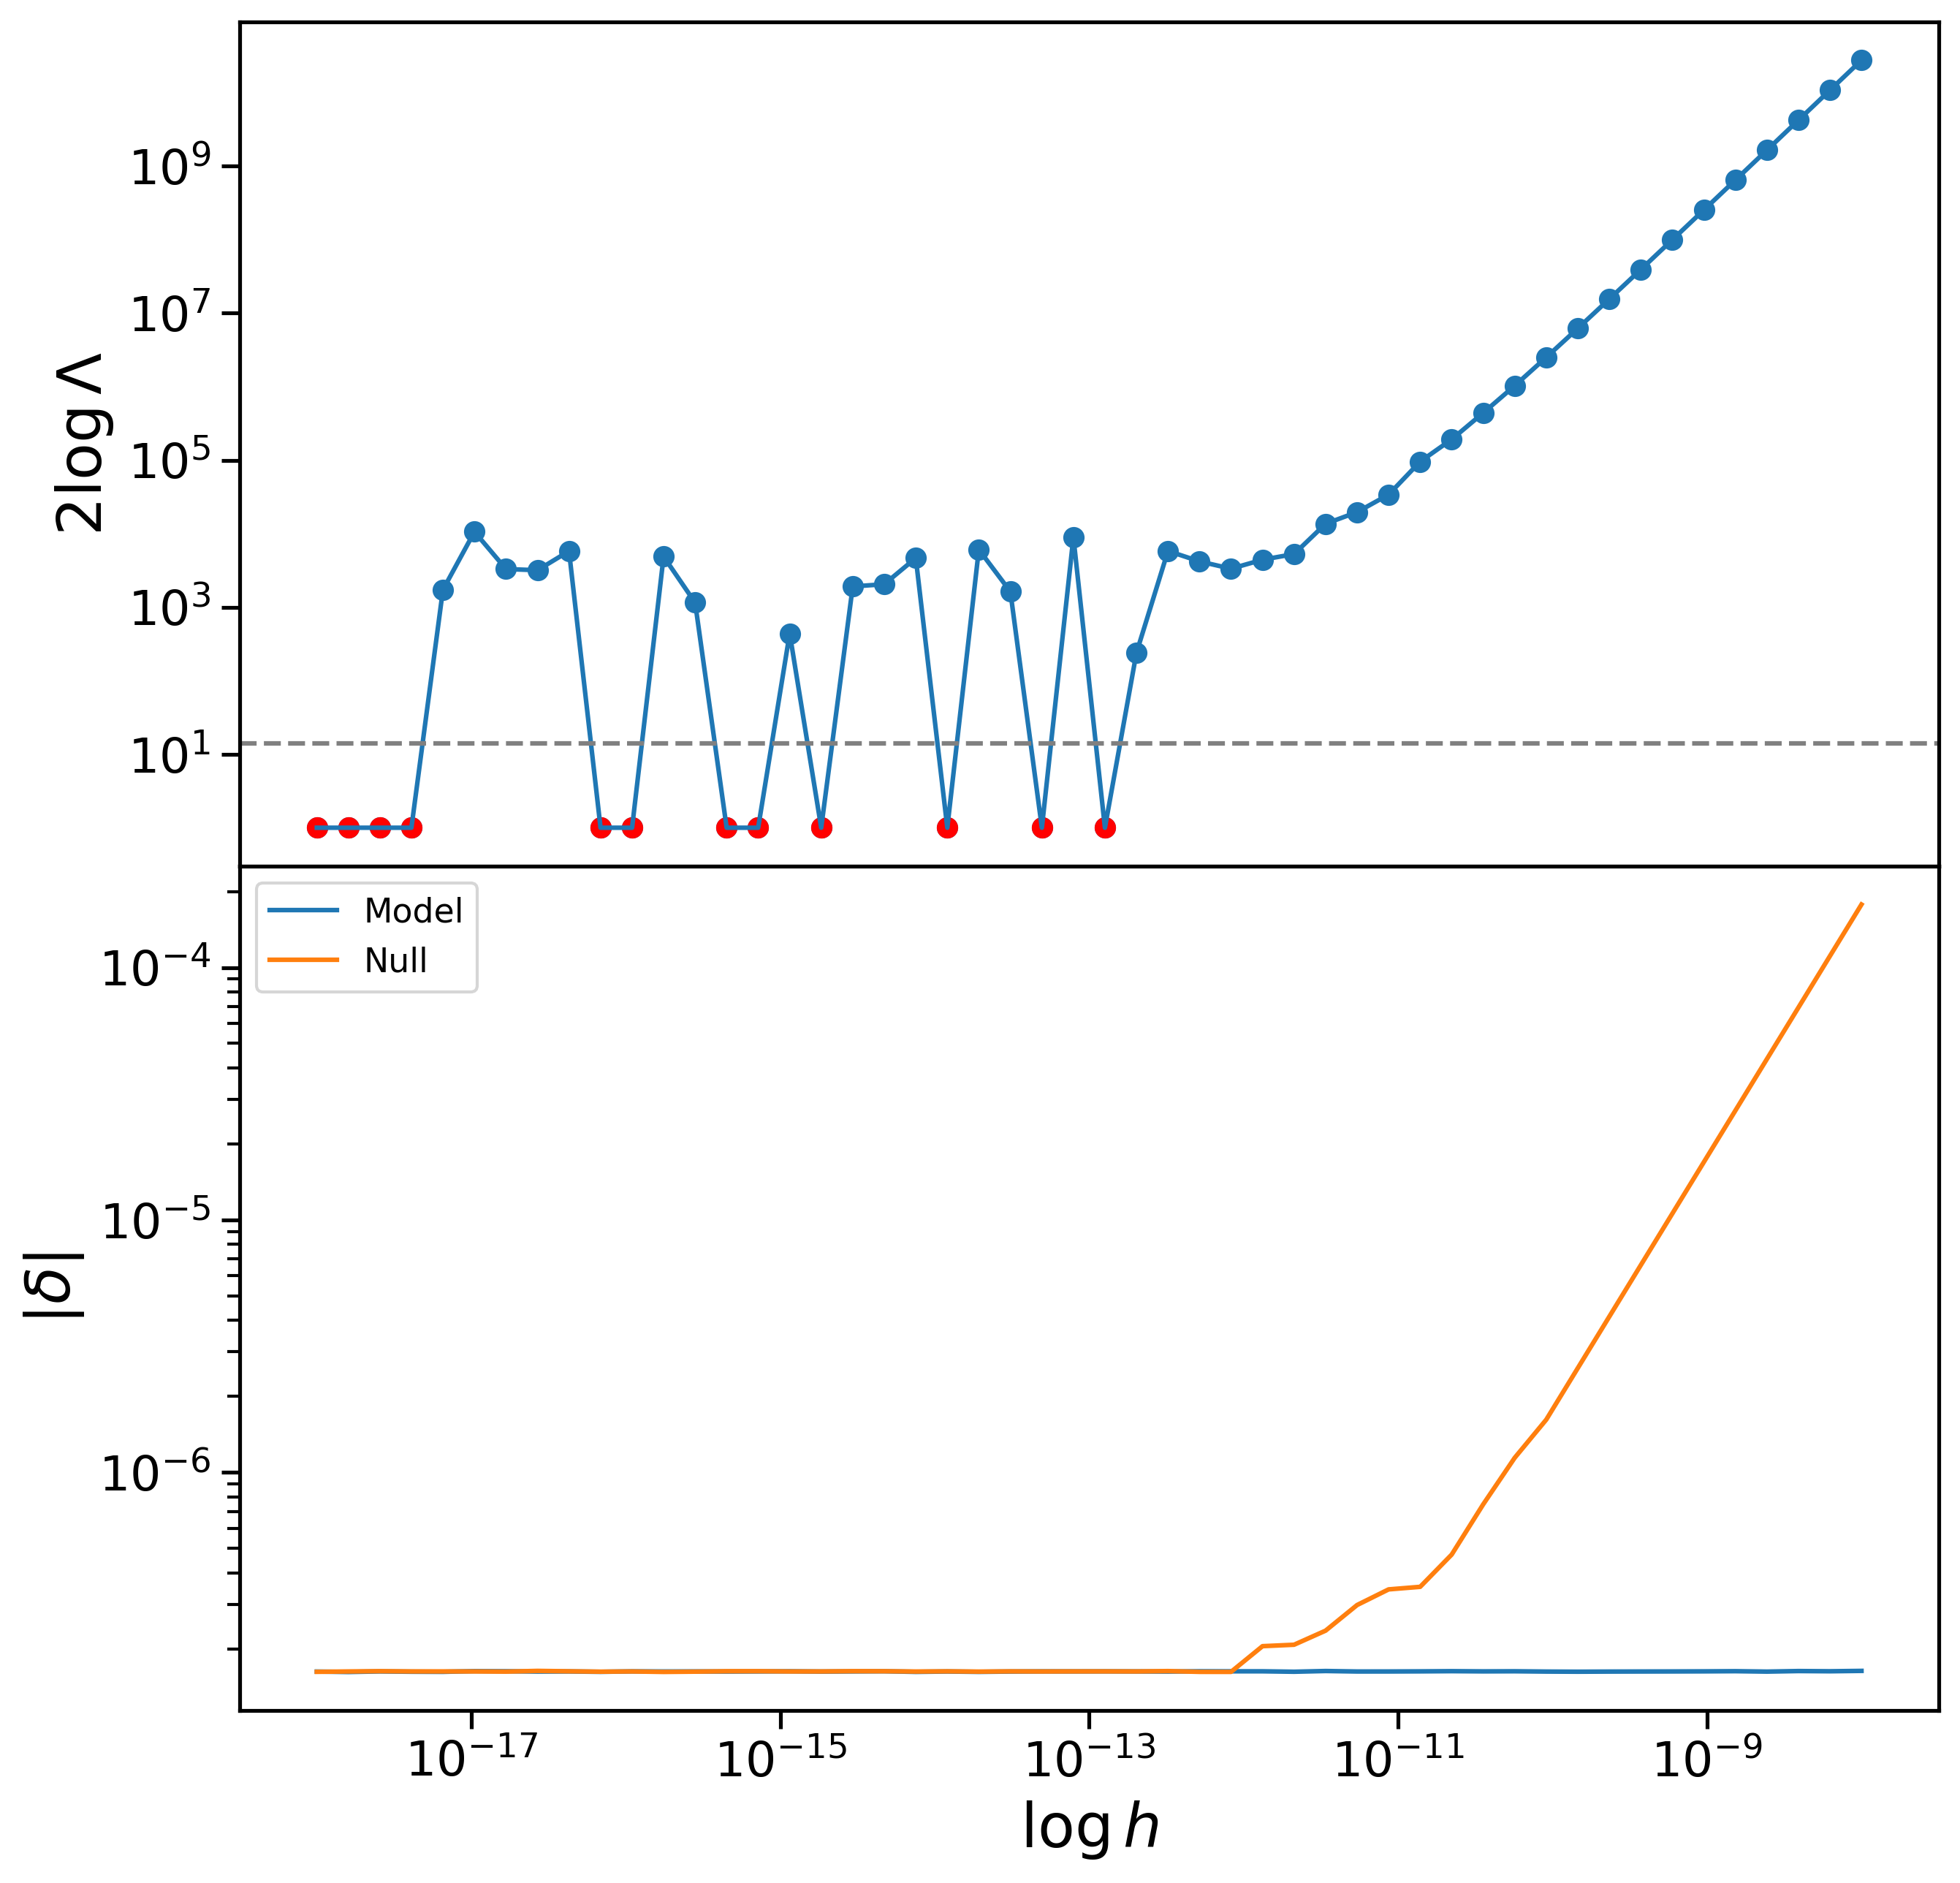
\includegraphics[width=0.8\textwidth]{images/SNR2}
	\caption{Variation of the test statistic (\textit{Top panel}) and the median state error (\textit{Bottom panel}) w.r.t GW strain. The grey horizontal line labels a test statistic of 14. Below $h \sim 10^{-12}$ the models cease to be consistently hierarchical - values with negative test statistics are set automatically $=1$ and marked with a red dot.}
	\label{fig:SNR}
\end{figure}

\begin{figure}
	\centering

	\begin{subfigure}[b]{0.475\textwidth}  
		\centering 
		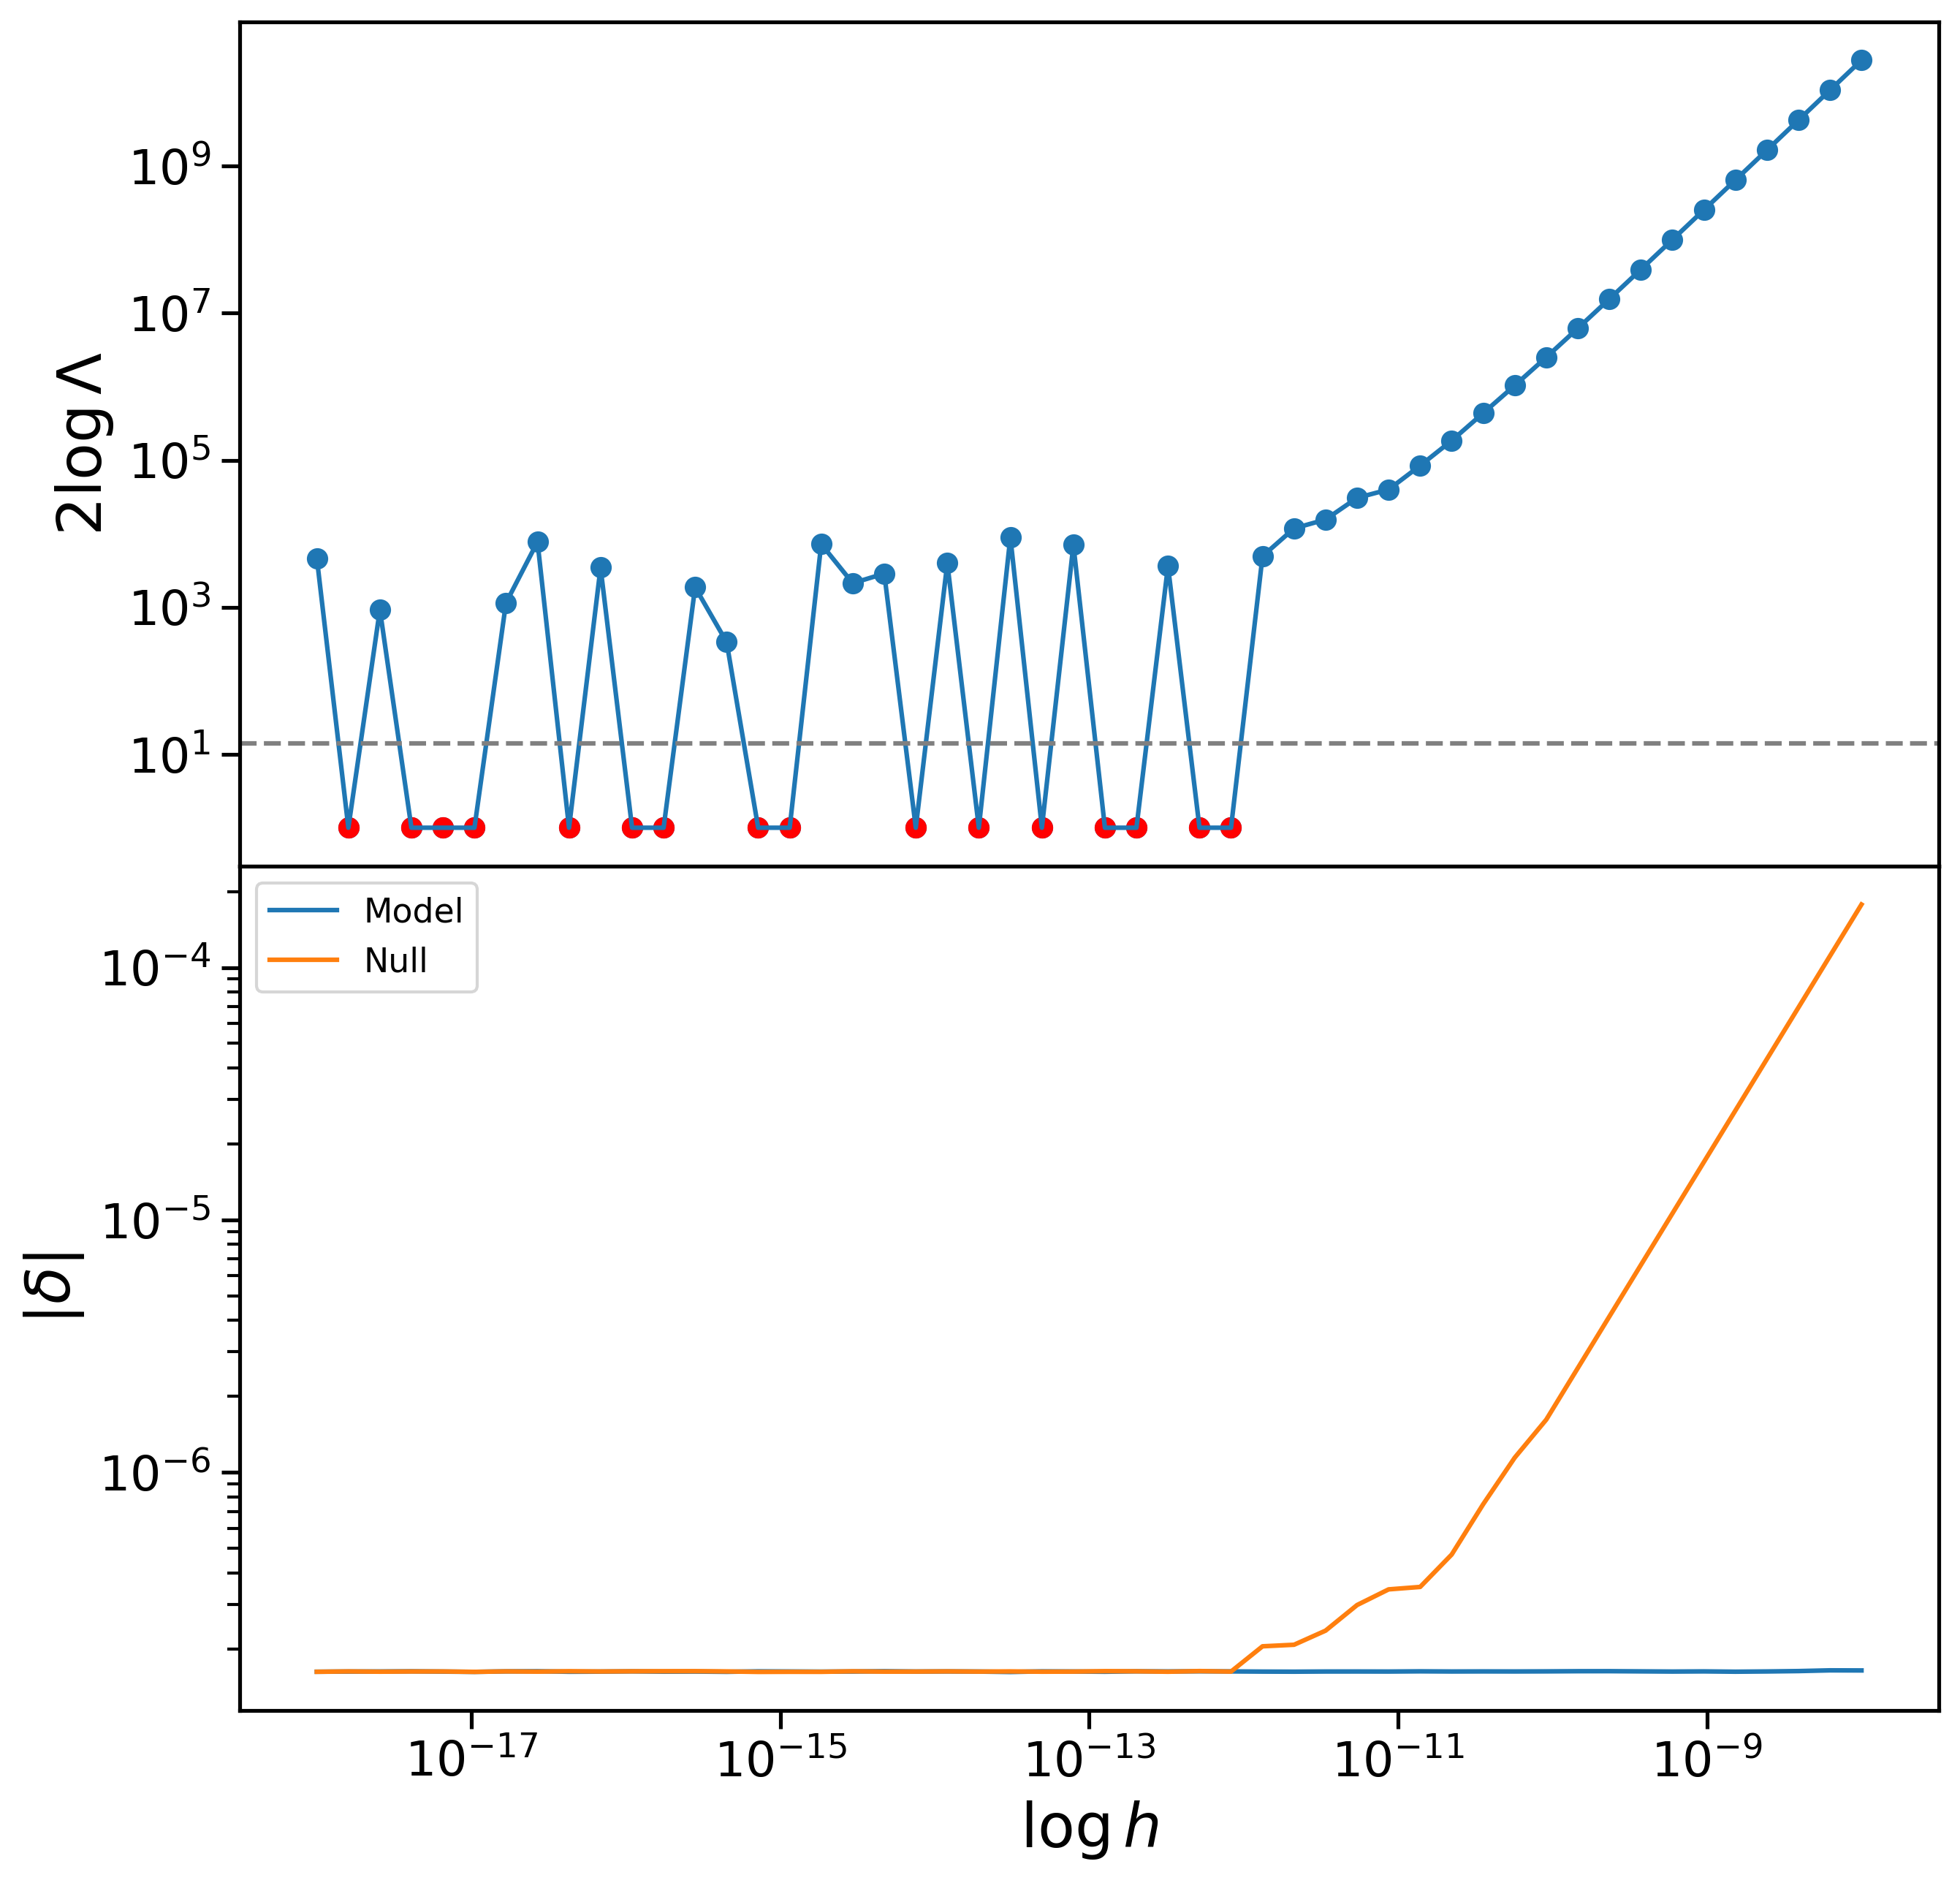
\includegraphics[width=\textwidth]{images/SNR2_differentnoise}
		\caption{Full PTA, different noise realisation}
		\label{fig:SNR2a}
	\end{subfigure}
	\vskip\baselineskip
	\begin{subfigure}[b]{0.475\textwidth}   
		\centering 
		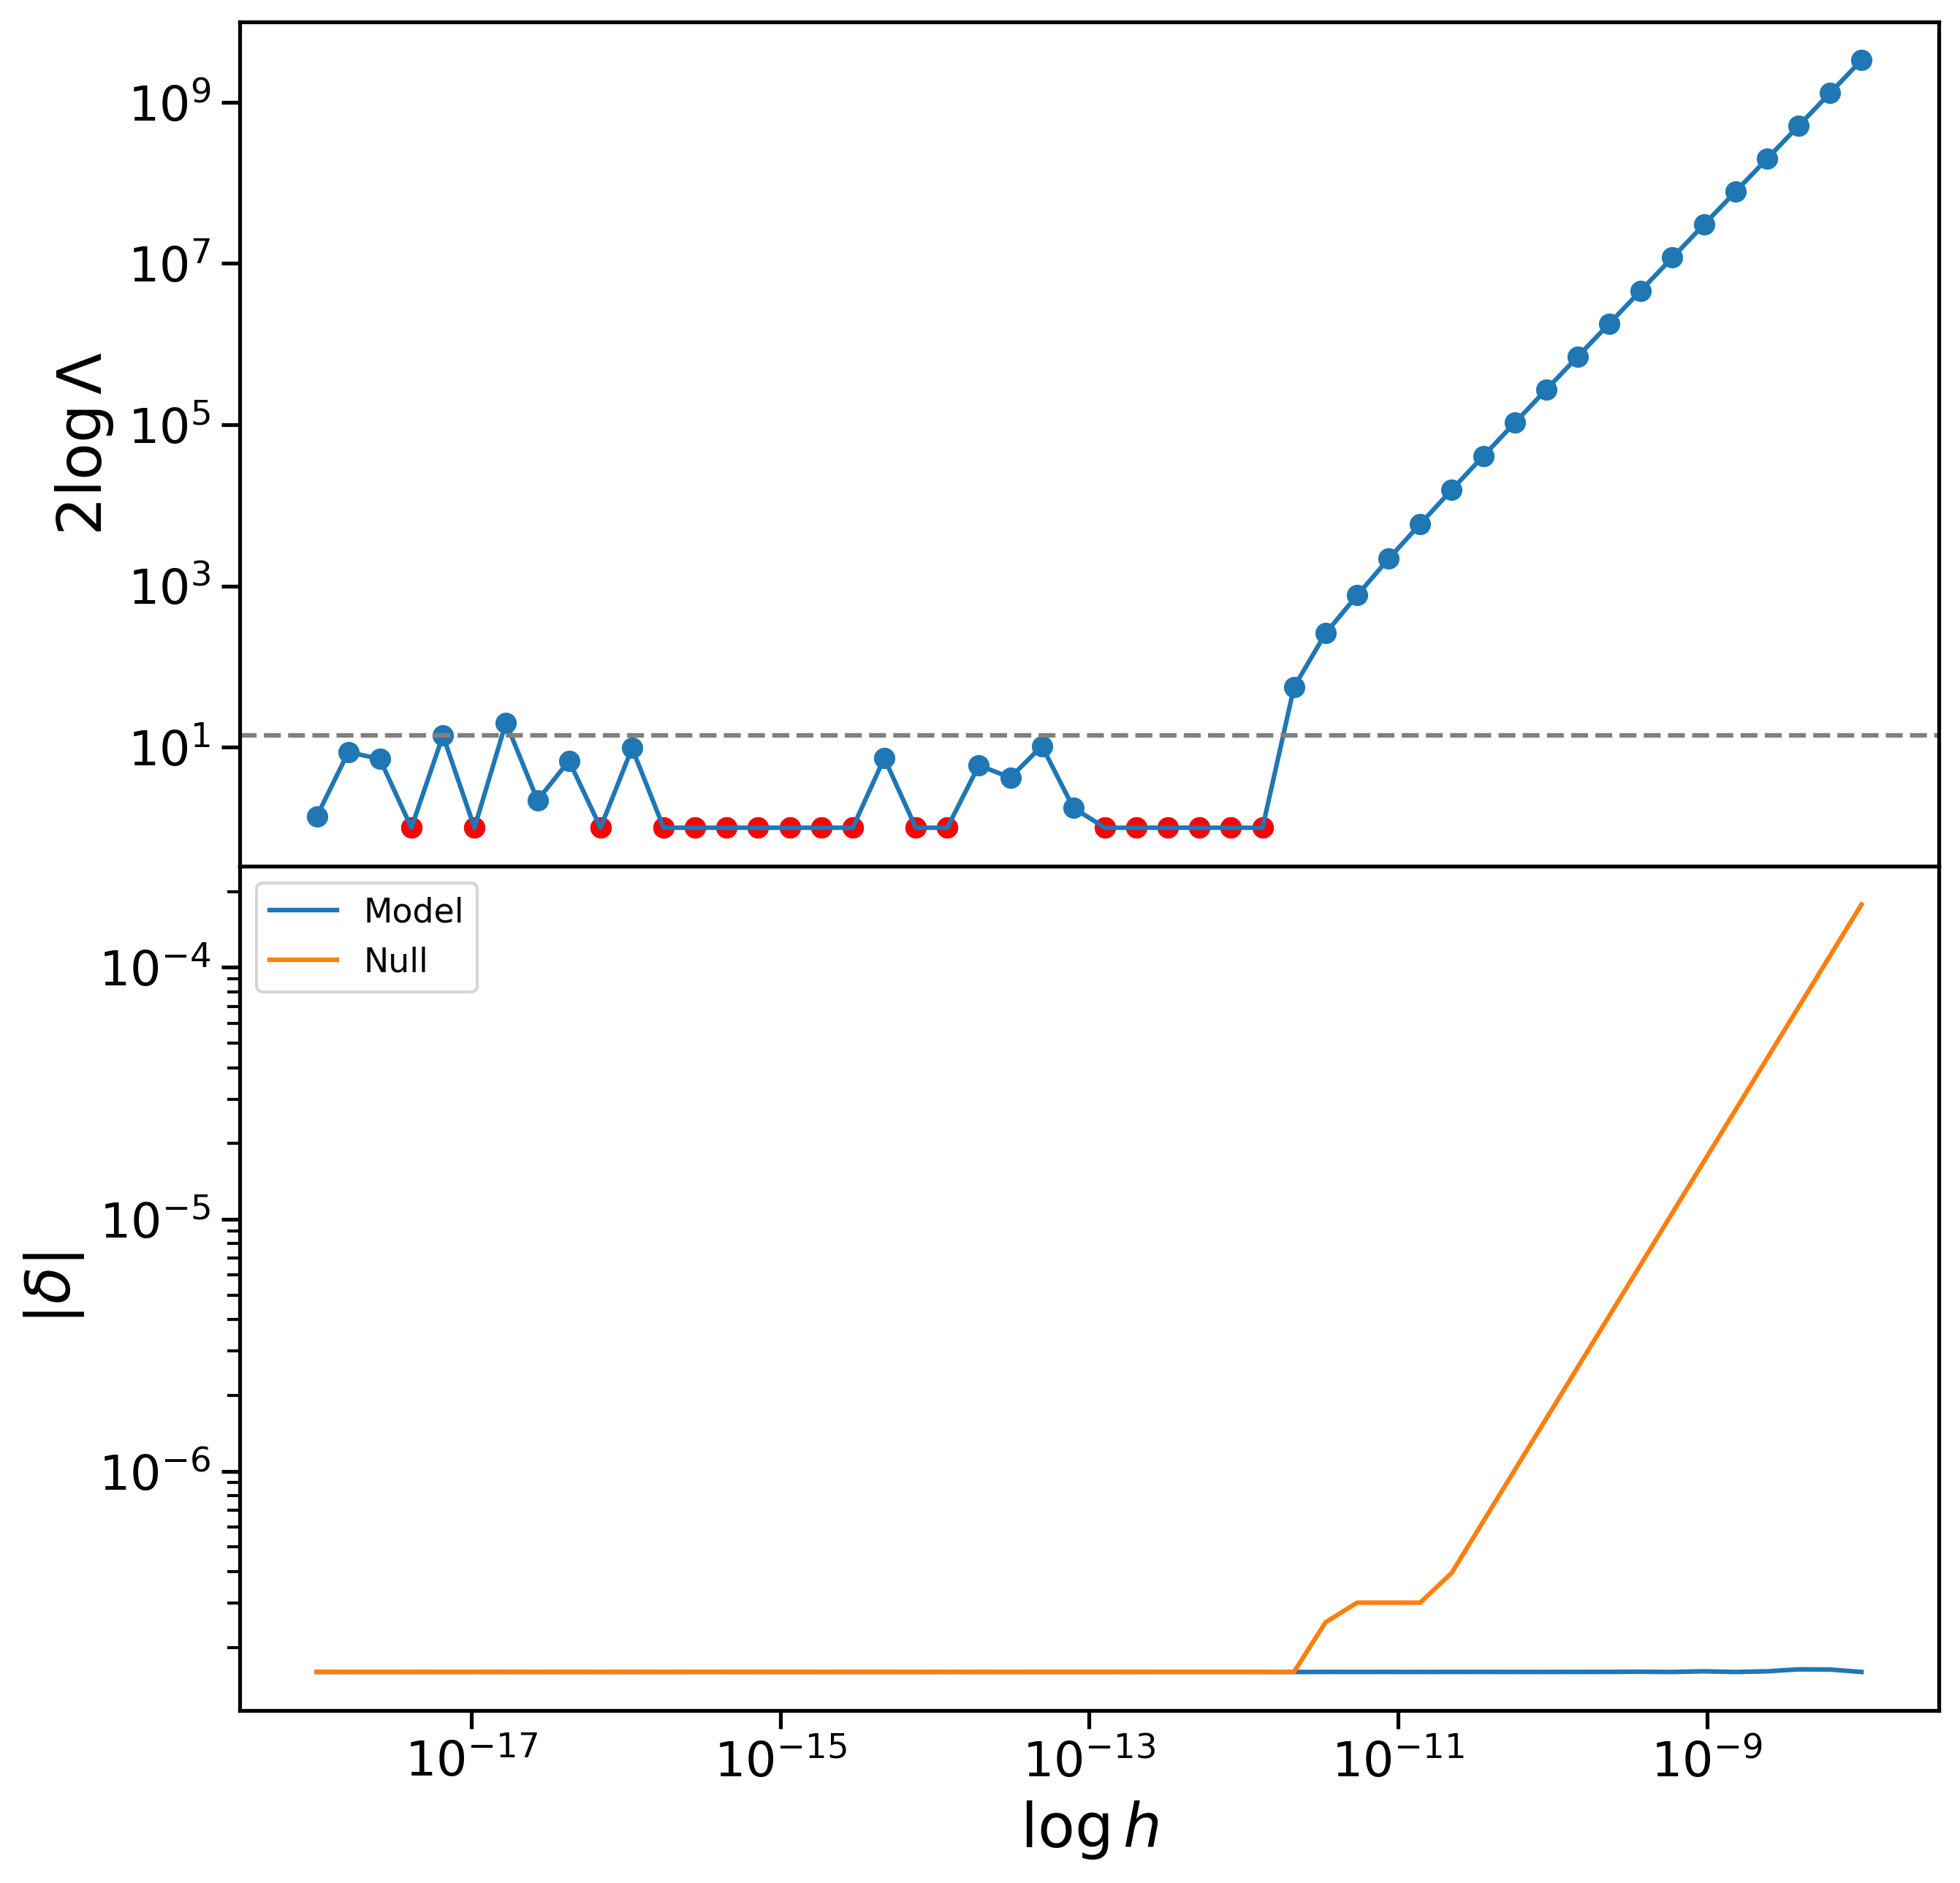
\includegraphics[width=\textwidth]{images/SNR2_frac02}
		\caption{Only using 20 \% of pulsars}  
		\label{fig:SNR2b}
	\end{subfigure}
	\hfill
	\begin{subfigure}[b]{0.475\textwidth}   
		\centering 
		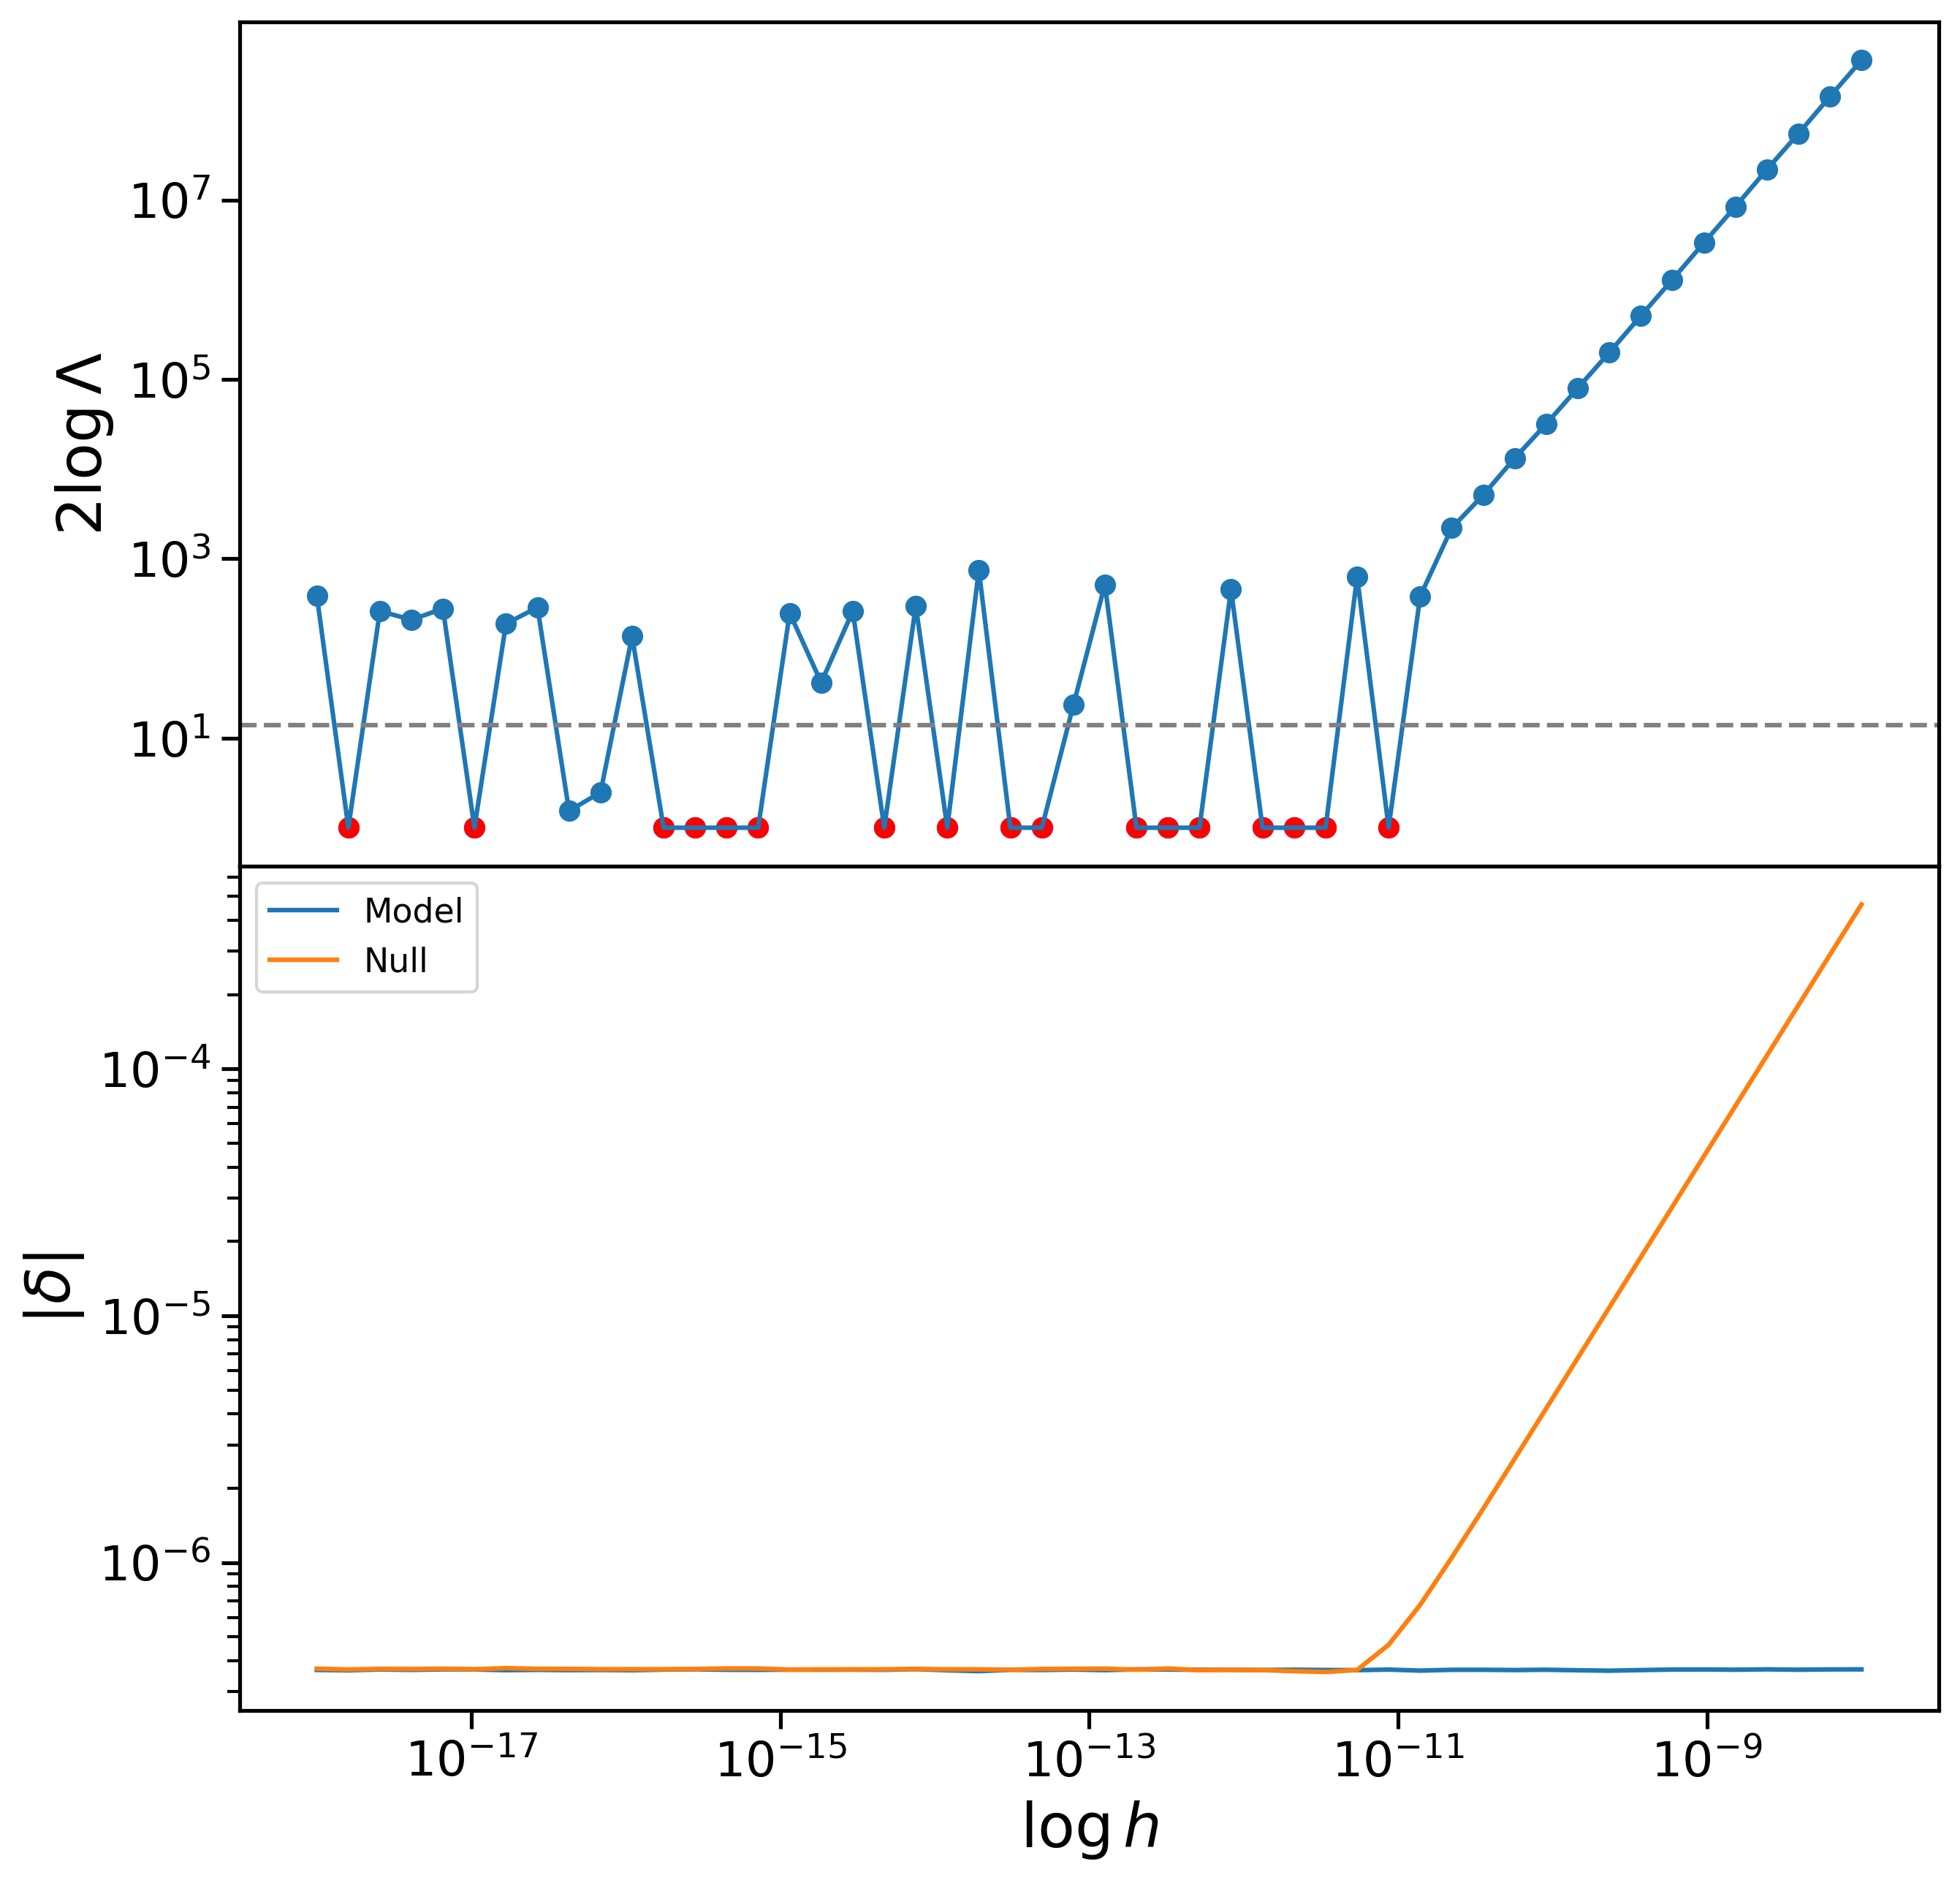
\includegraphics[width=\textwidth]{images/SNR2_n2}
		\caption{Only using 2 pulsars.}   
		\label{fig:SNR2c}
	\end{subfigure}
	\caption{As Figure 5, but for different noises and numbers of pulsars}
	\label{SNR2}
\end{figure}



 
 \newpage 
 \section{Caveats and questions}
 
 \begin{enumerate}
 	
 	\item We should really do this using a ``proper" language and enforce consistent number formats. We are using the Python long double, but there is some uncertainty around how e.g. linear algebra operations in Python handle these formats - do they just get rounded to doubles?  
 	
 	\item We have assumed that all pulsars have $n=3$. What about some distribution?
 	
 	\item We have only considered a single GW source at a particular location, polarisation, etc. What about others?
 	
 	\item We have focused only on a monochromatic GW source. This is probably not a bad approximation, but maybe we can include some process noise on the phase evolution too?
 	
 	 \item We assume all pulsars have observations taken at the same time
 	
 	\item How reasonable are our noises? For instance, what is a reasonable measurement noise on the frequency evolution of a MSP?
 	
 	 \item What about doing a full Bayesian search using e.g. Bilby to get a Bayes ratio?
 	
 	 \item How good/bad an assumption is it that $\hat{\theta} \sim \theta$ for our likelihood ratio test?
 \end{enumerate}
 

\end{document}